\documentclass[xcolor=dvipsnames]{beamer}

\usepackage[utf8x]{inputenc}
\usepackage[slovak]{babel}
\usepackage{amsfonts}
\usepackage{amsmath}
\usepackage{epstopdf}
\usepackage{graphicx}
\DeclareGraphicsExtensions{.png,.pdf,.eps}
\usepackage{stmaryrd}
\usepackage{multimedia}
\usepackage{hyperref}
\usepackage{float}
\usepackage{booktabs}

\newcommand{\B}{{\mathcal{B}}}
\newcommand{\ii}{{\boldsymbol {i}}}
\newcommand{\jj}{{\boldsymbol {j}}}
\newcommand{\kk}{{\boldsymbol {k}}}

\definecolor{Present}{RGB}{160,160,160}
\definecolor{PresentNadpis}{RGB}{0,0,0}
\definecolor{FrameNadpis}{RGB}{0,0,0}
\definecolor{BlockNadpis}{RGB}{237,28,36}
\definecolor{BlockNadpisPodklad}{RGB}{220,220,220}
\definecolor{BlockPodklad}{RGB}{255,255,255}

\usecolortheme[named=Present]{structure} 
\usetheme{Montpellier} 
\setbeamertemplate{blocks}[rounded][shadow=true]
\setbeamertemplate{navigation symbols}{} 

\setbeamercolor{title}{fg=PresentNadpis}
\setbeamercolor{frametitle}{fg=FrameNadpis}
\setbeamercolor{block body}{bg=BlockPodklad} 
\setbeamercolor{block title}{bg=BlockNadpisPodklad}
\setbeamercolor{block title}{fg=BlockNadpis}

\begin{document}

\begin{frame}[plain]{}
	\begin{center}
		\Huge\textsc{\Huge 1.}

		\textsc{\huge Spectra displayed in same scale}
	\end{center}
\end{frame}

\begin{frame}[plain]{}
\begin{figure}[htb]
	\centering
	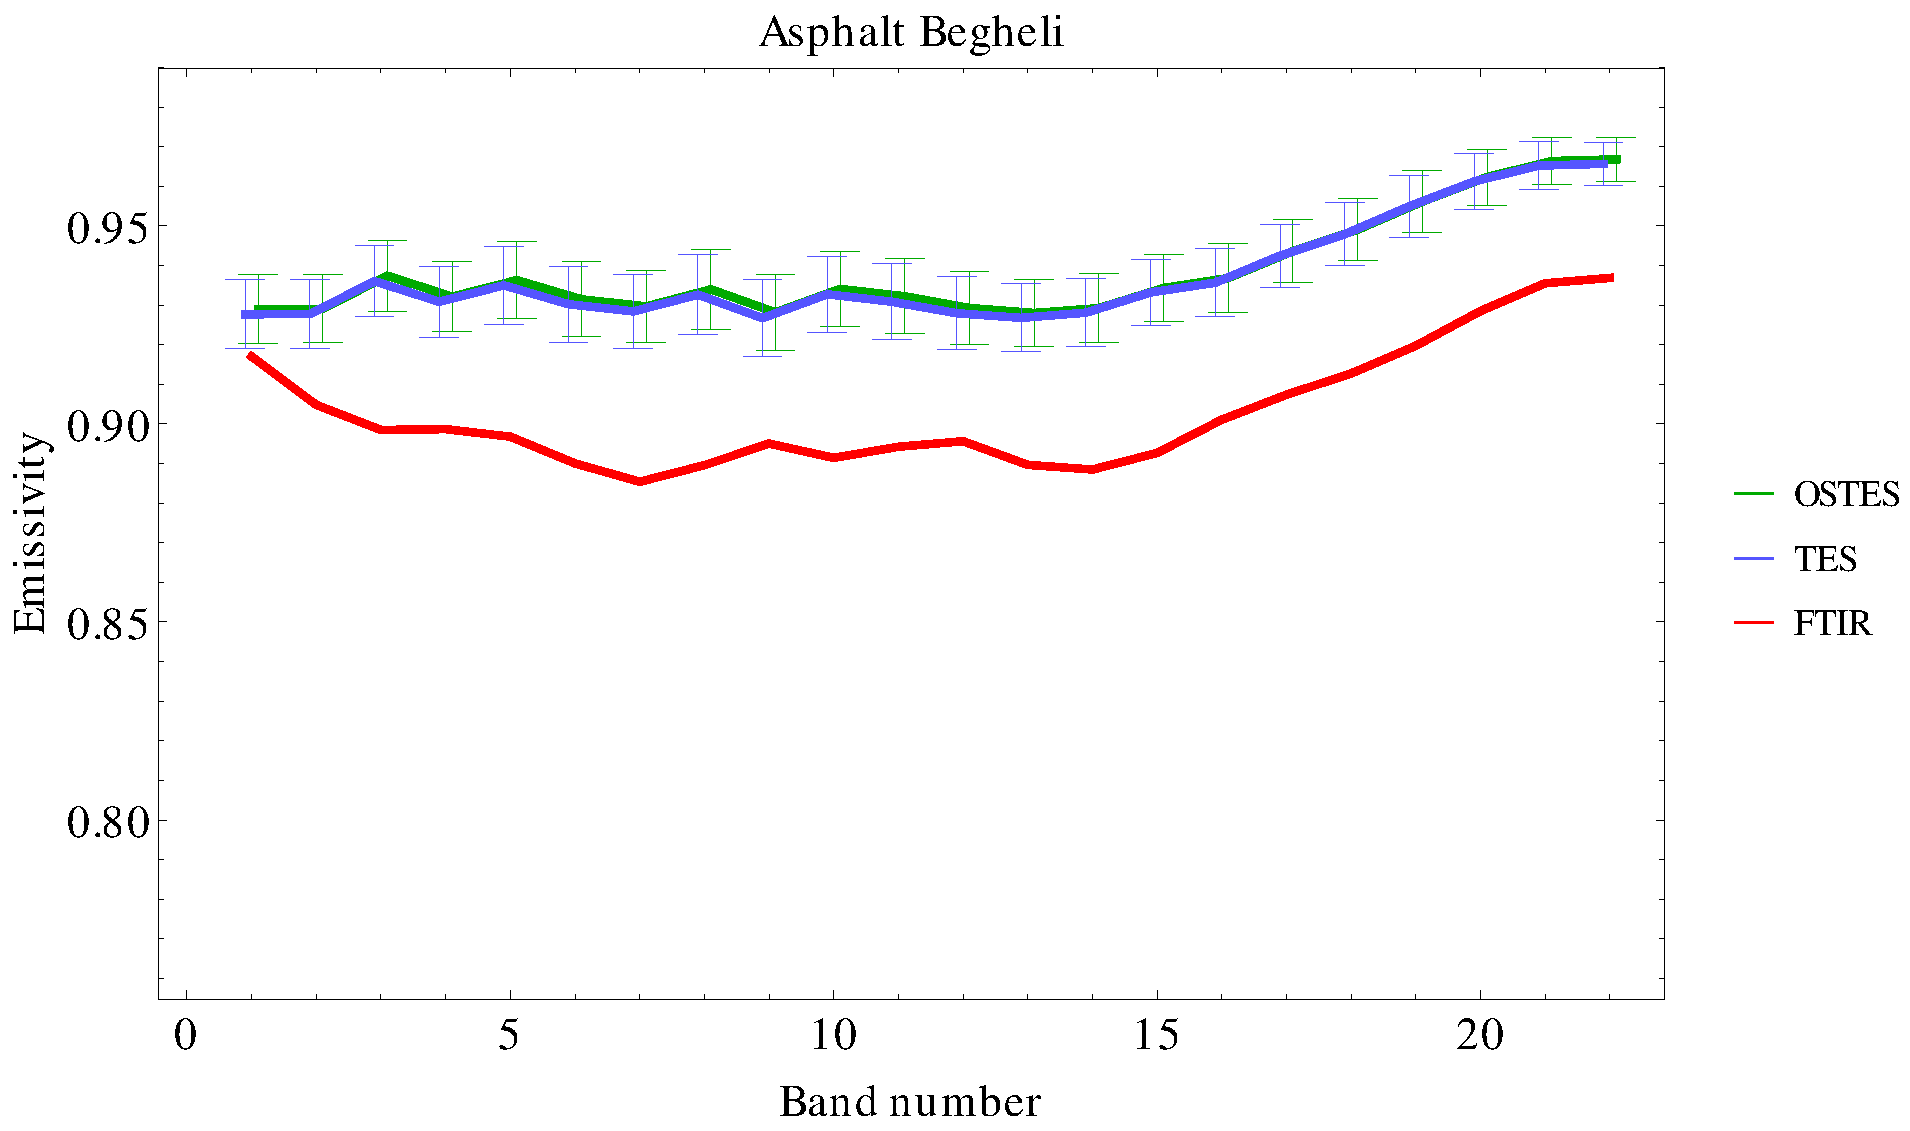
\includegraphics[scale=0.35]{AsphaltBegheli.pdf}
\end{figure}
\end{frame}

\begin{frame}[plain]{}
\begin{figure}[htb]
	\centering
	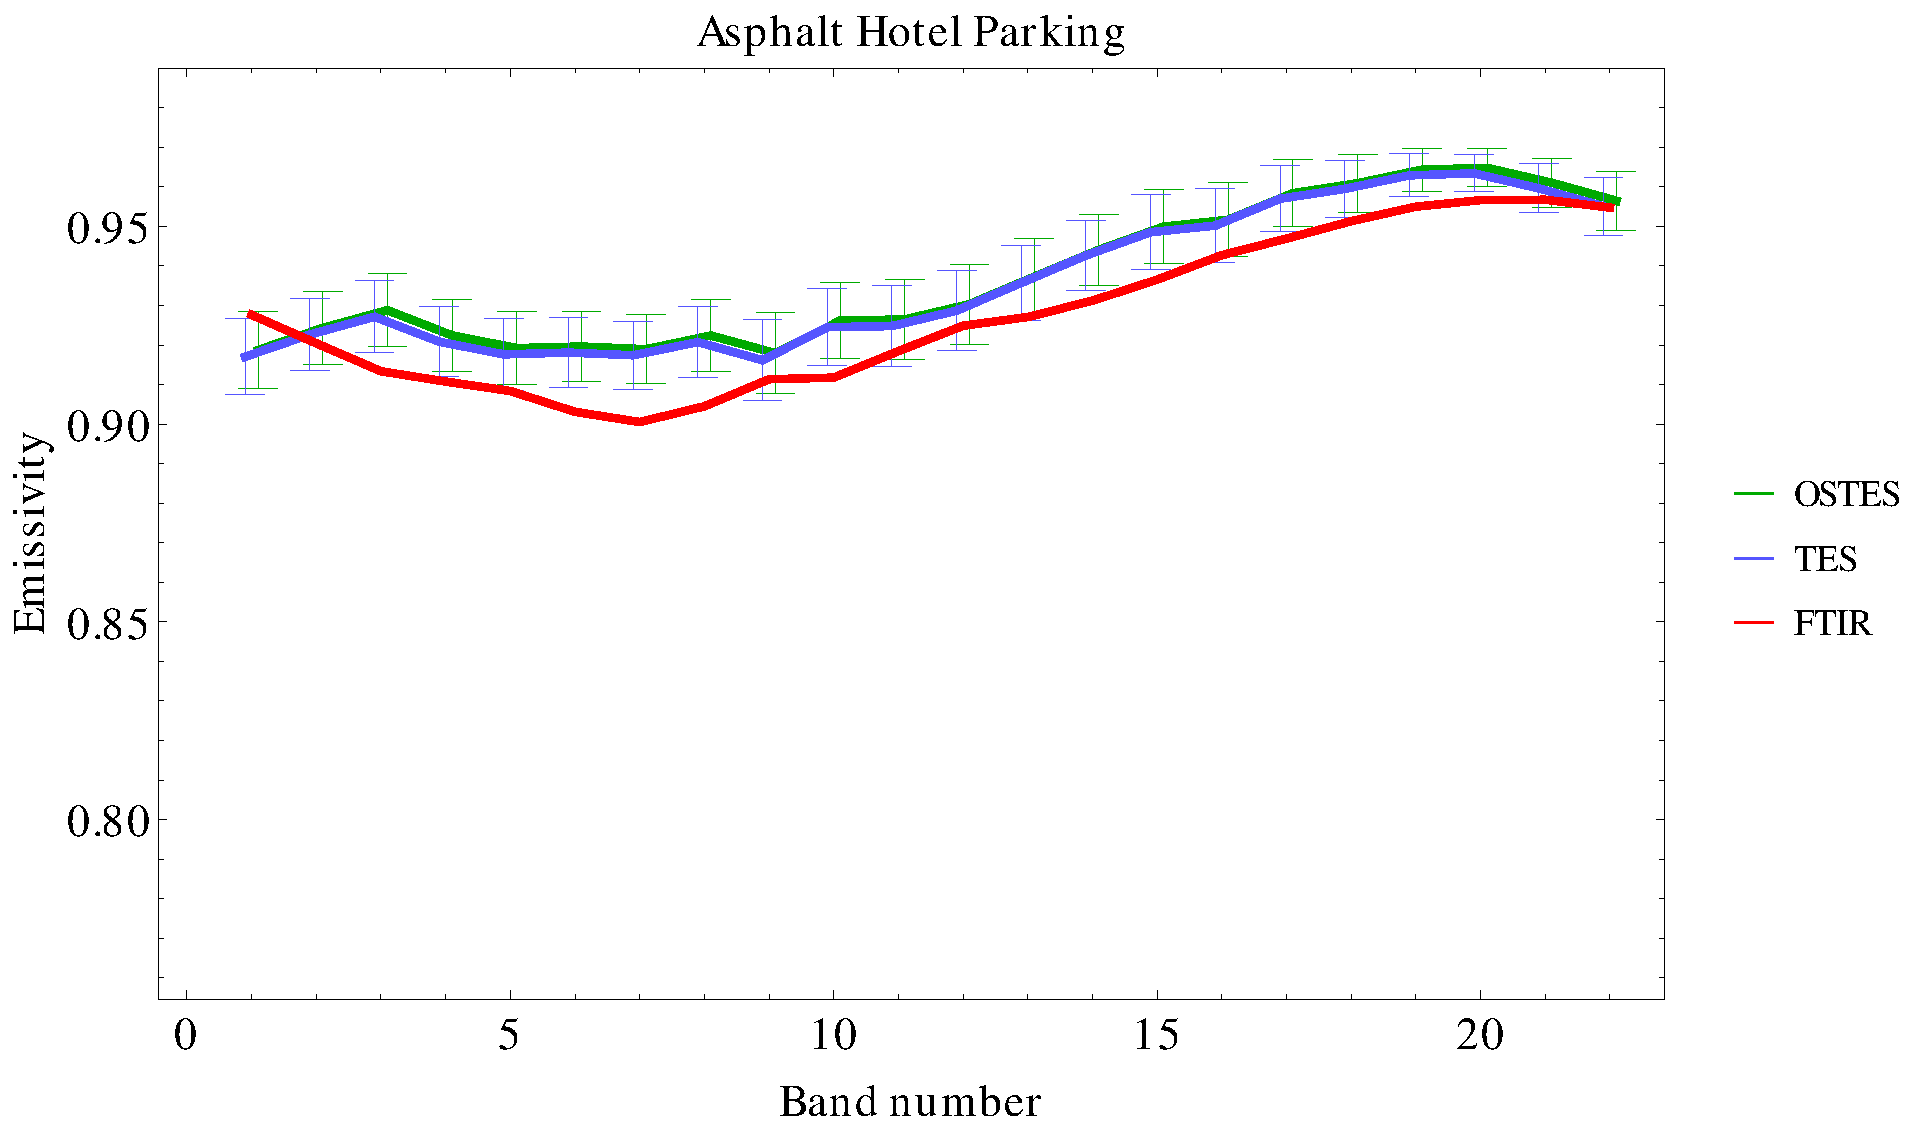
\includegraphics[scale=0.35]{AsphaltHotelParking.pdf}
\end{figure}
\end{frame}

\begin{frame}[plain]{}
\begin{figure}[htb]
	\centering
	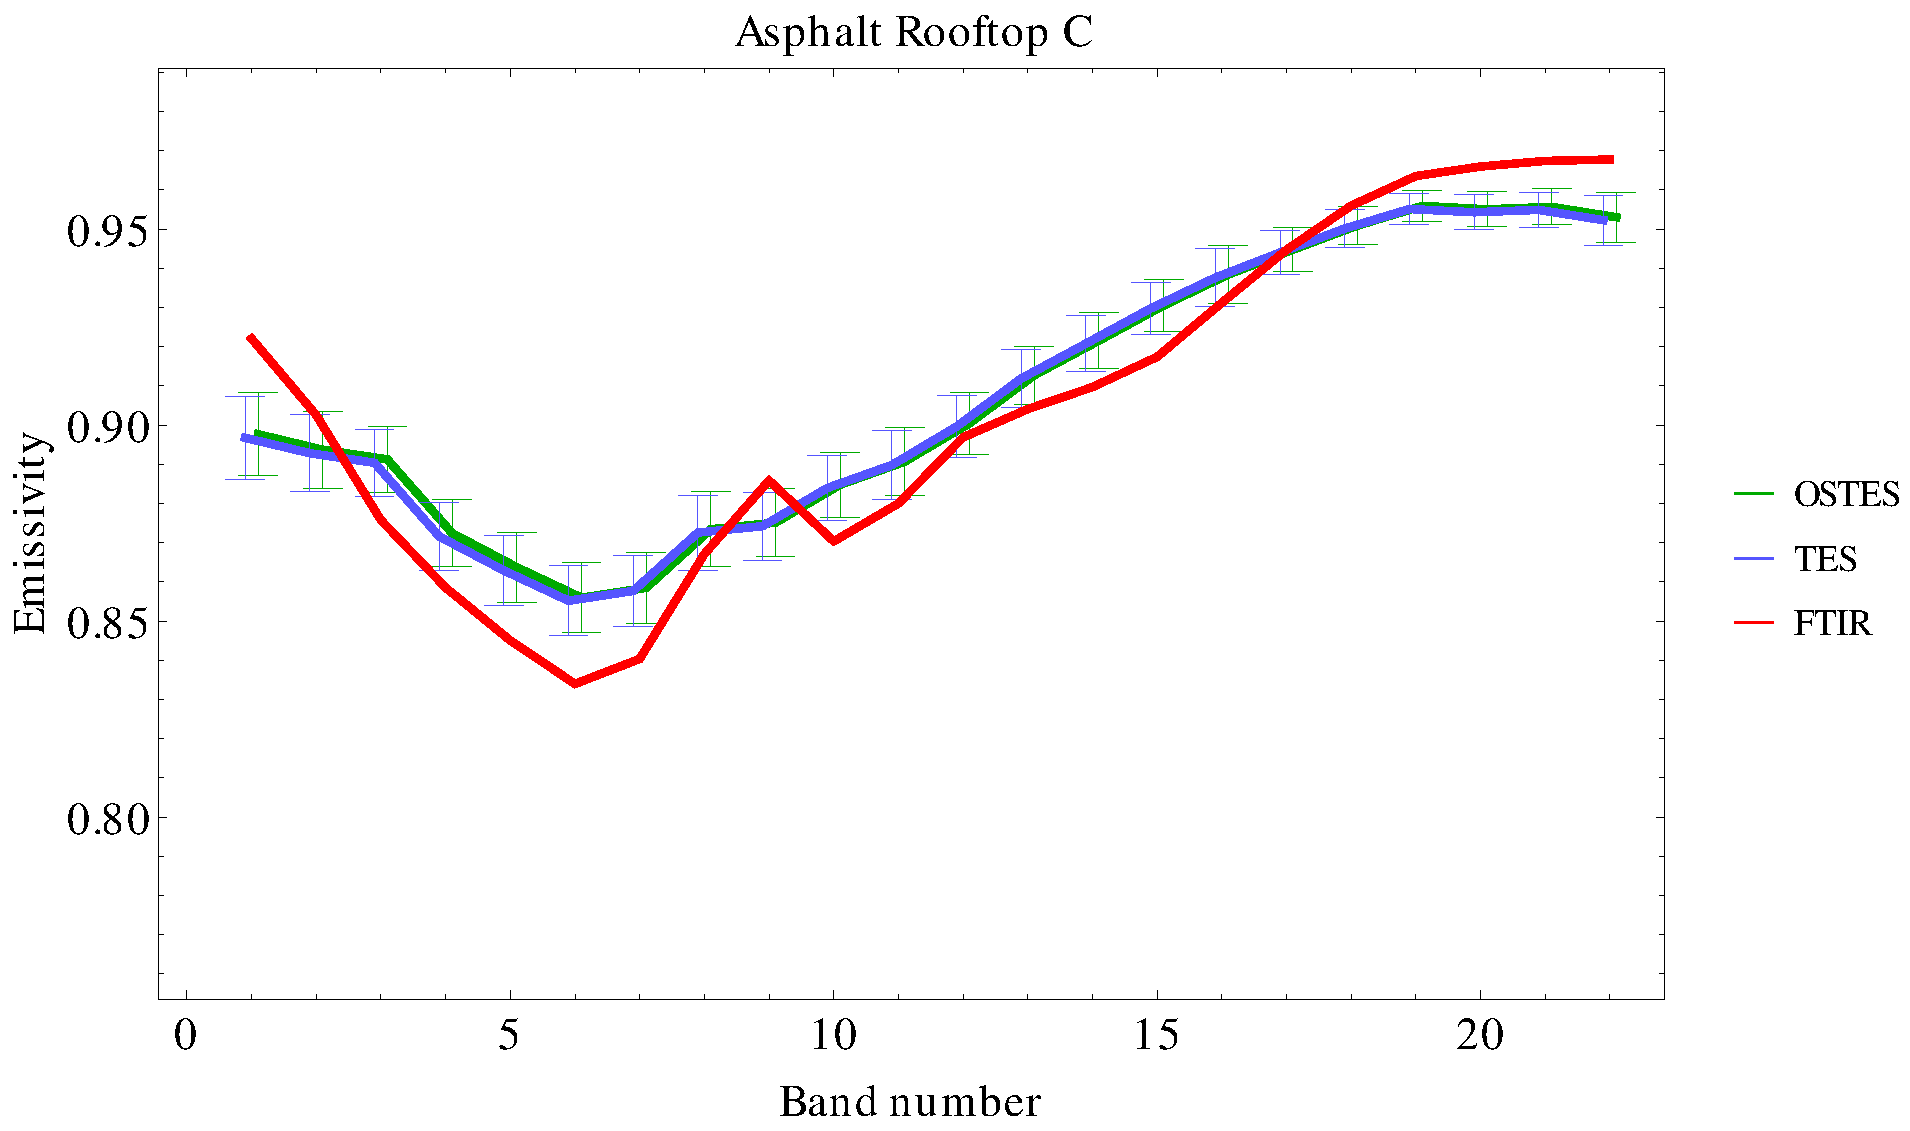
\includegraphics[scale=0.35]{AsphaltRooftopC.pdf}
\end{figure}
\end{frame}

\begin{frame}[plain]{}
\begin{figure}[htb]
	\centering
	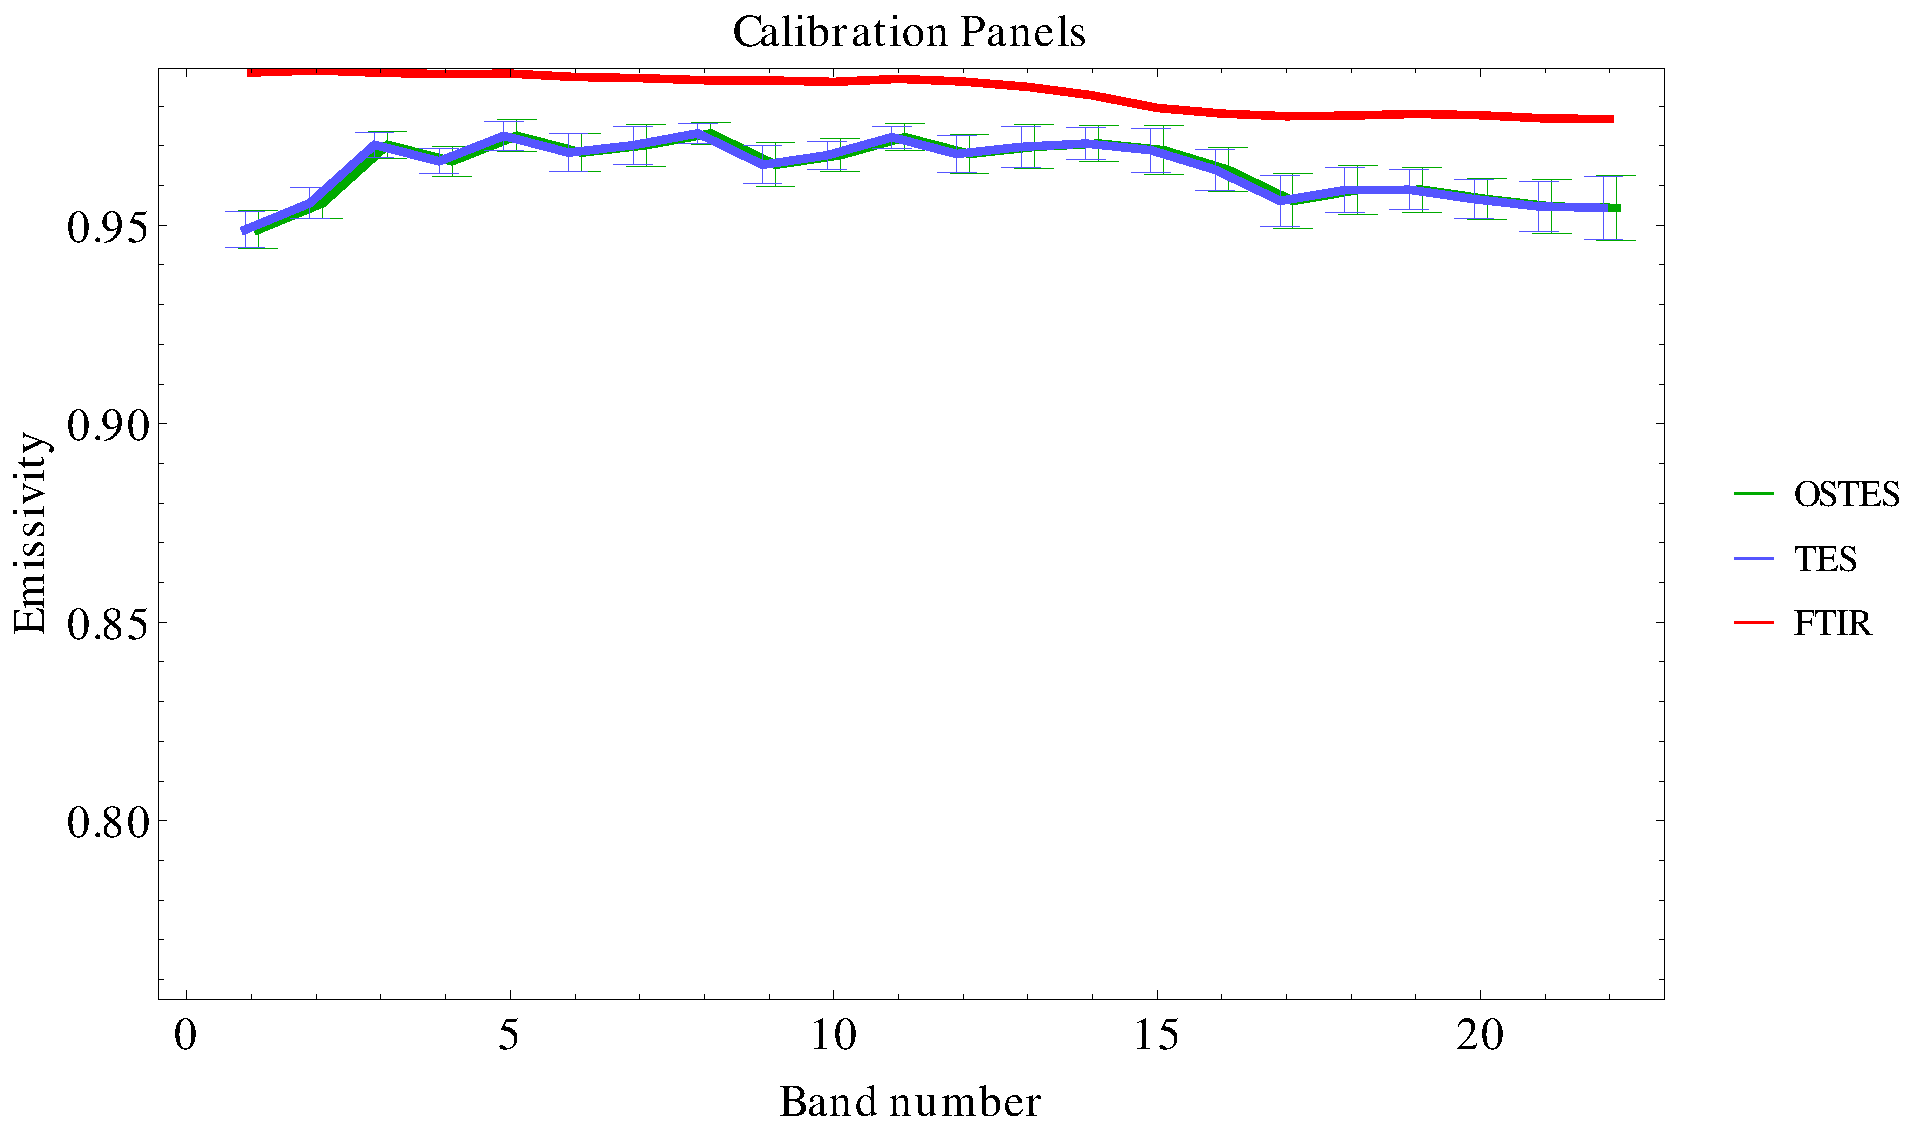
\includegraphics[scale=0.35]{CalibrationPanels.pdf}
\end{figure}
\end{frame}

\begin{frame}[plain]{}
\begin{figure}[htb]
	\centering
	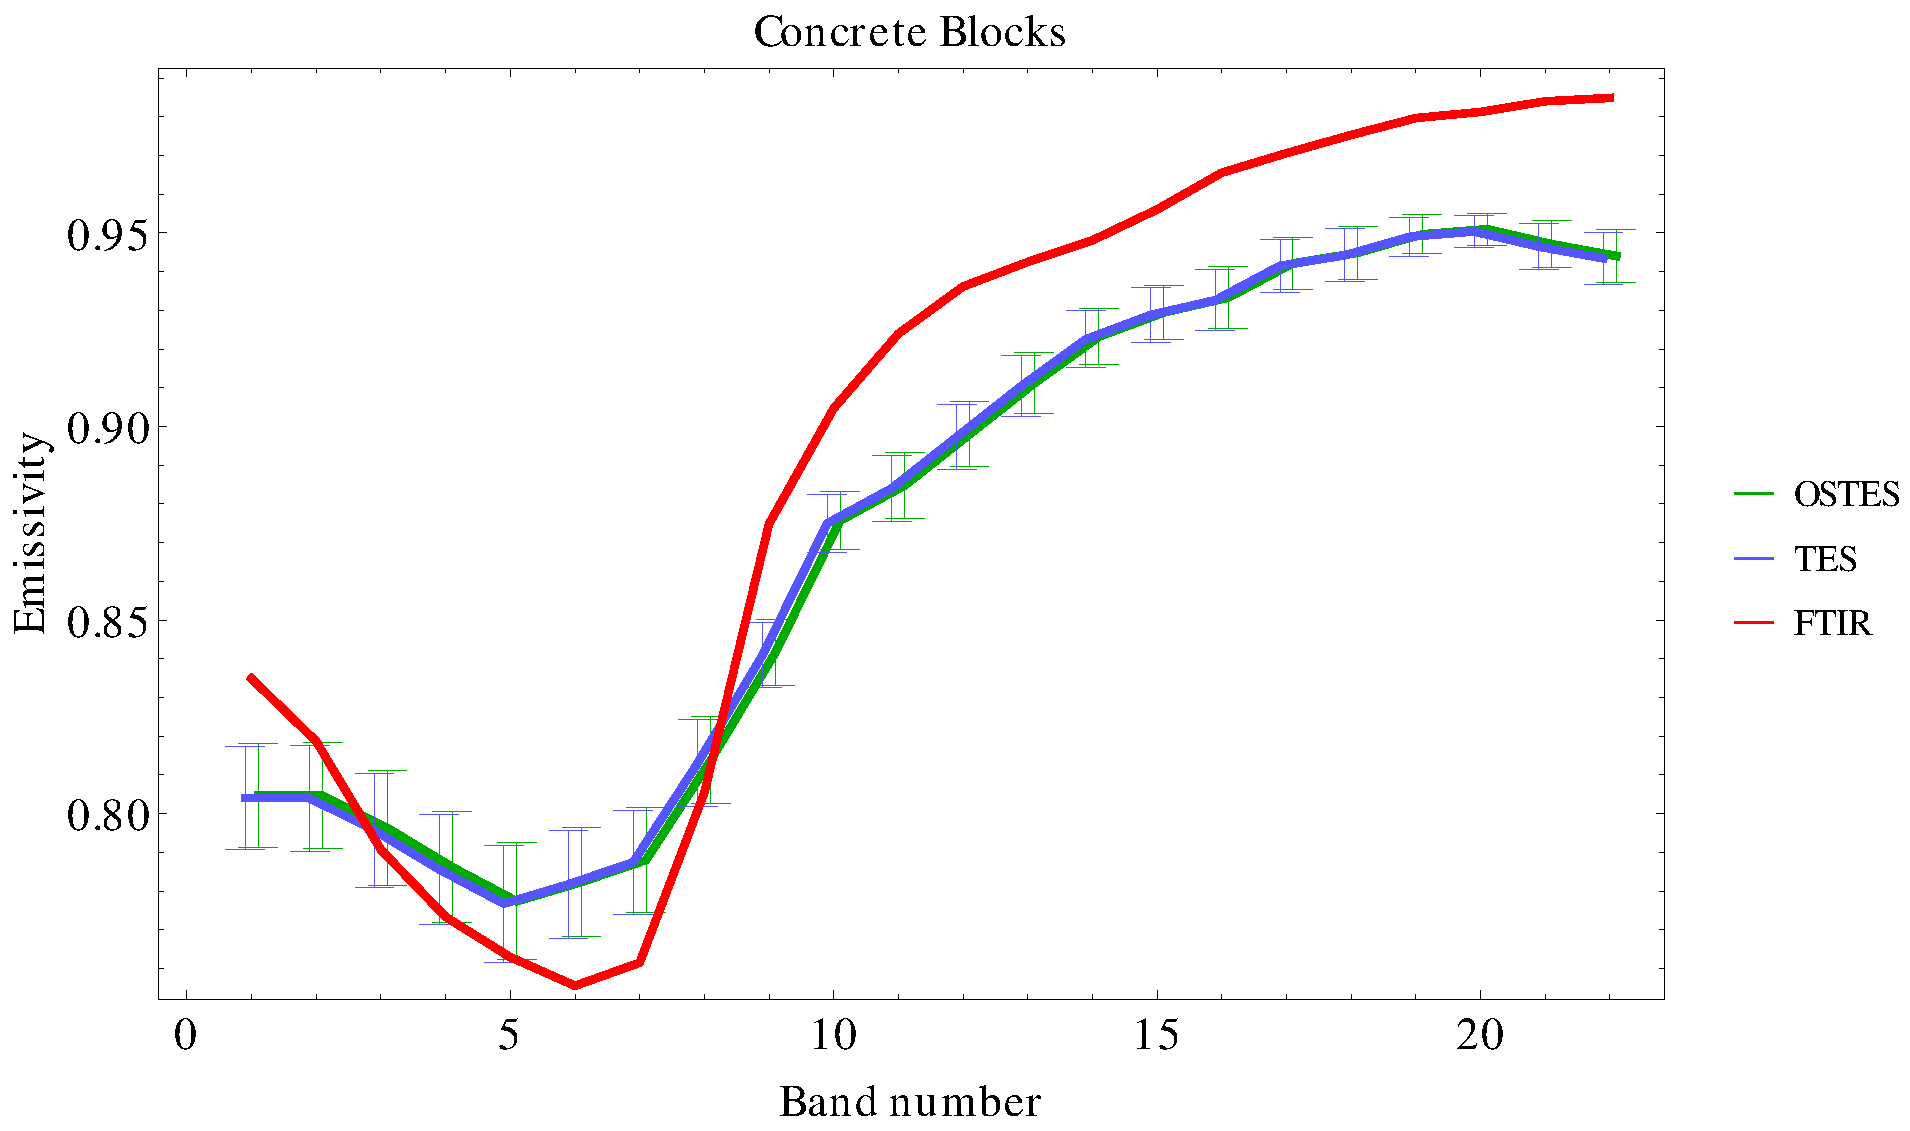
\includegraphics[scale=0.35]{ConcreteBlocks.pdf}
\end{figure}
\end{frame}

\begin{frame}[plain]{}
\begin{figure}[htb]
	\centering
	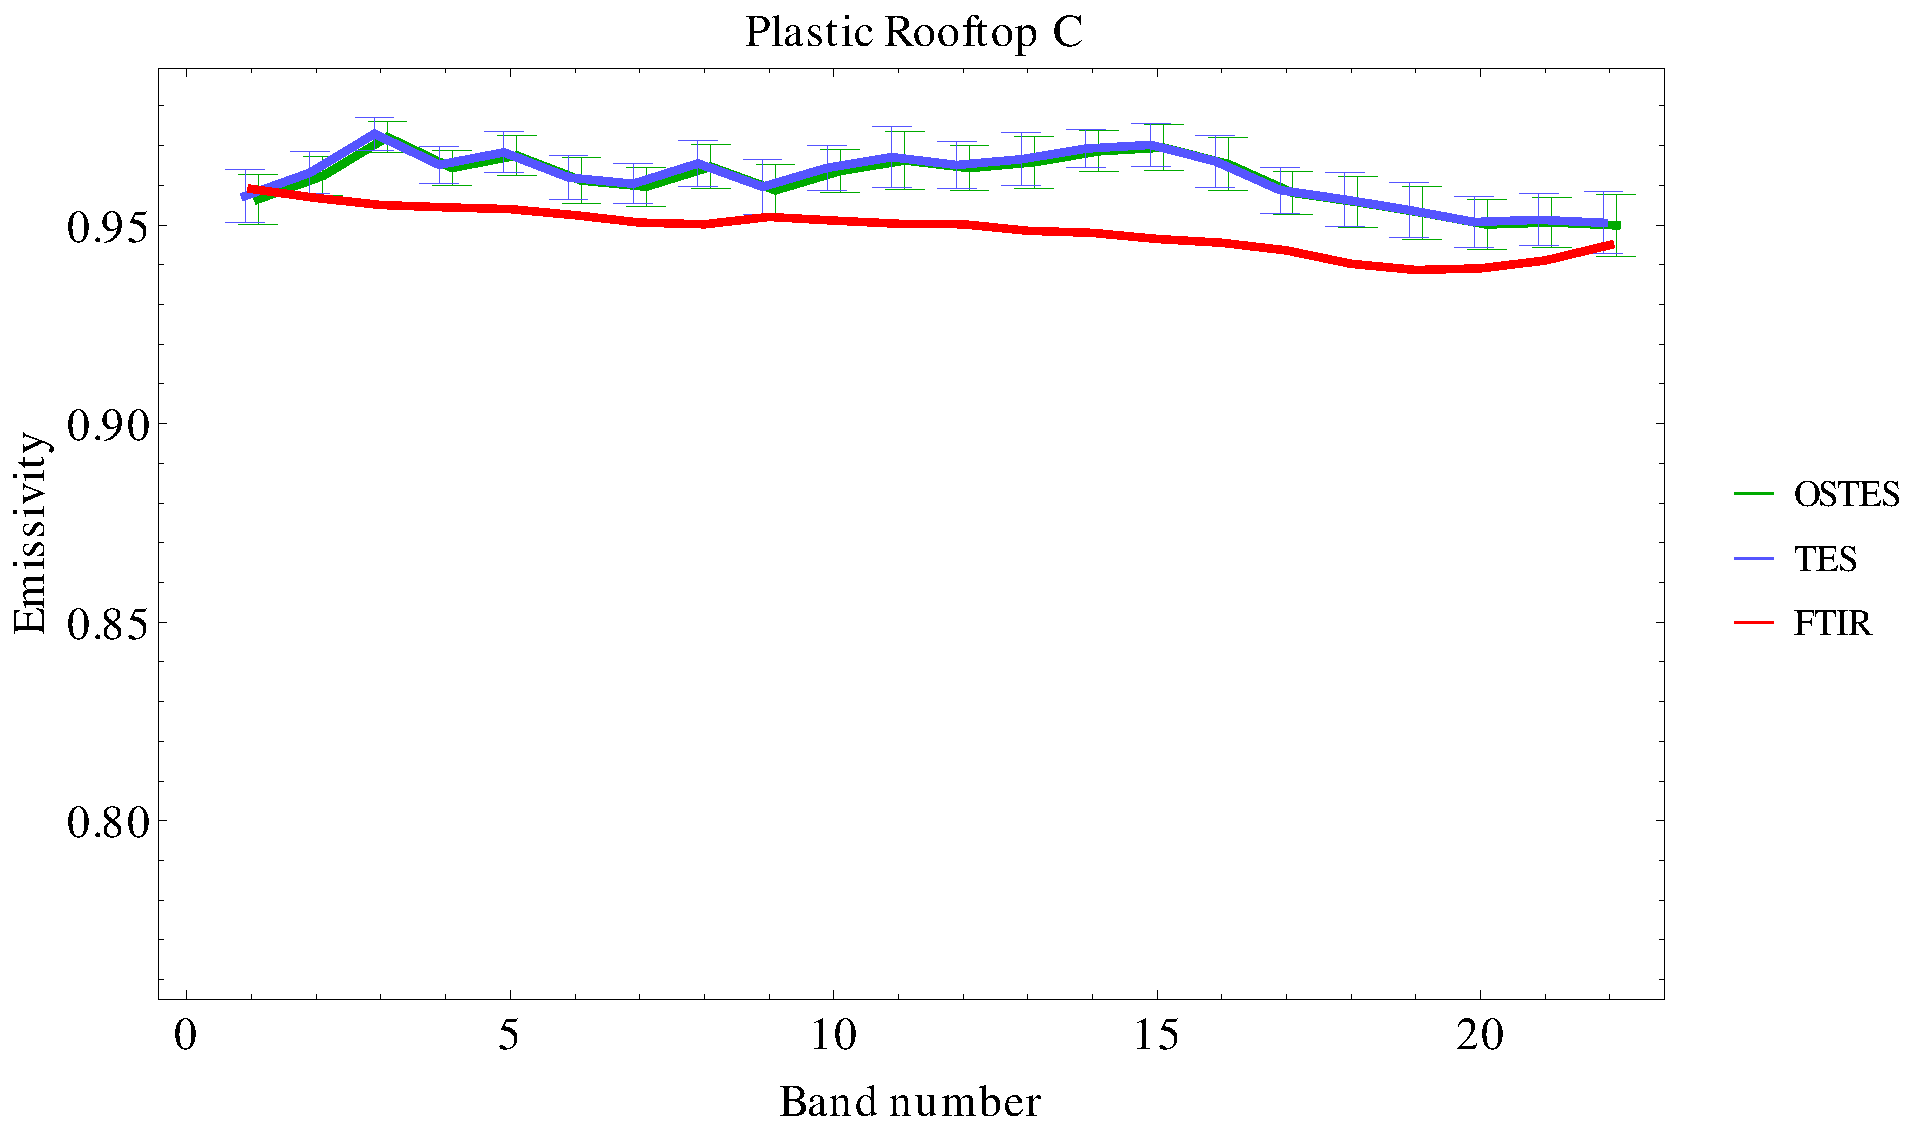
\includegraphics[scale=0.35]{PlasticRooftopC.pdf}
\end{figure}
\end{frame}

\begin{frame}[plain]{}
\begin{figure}[htb]
	\centering
	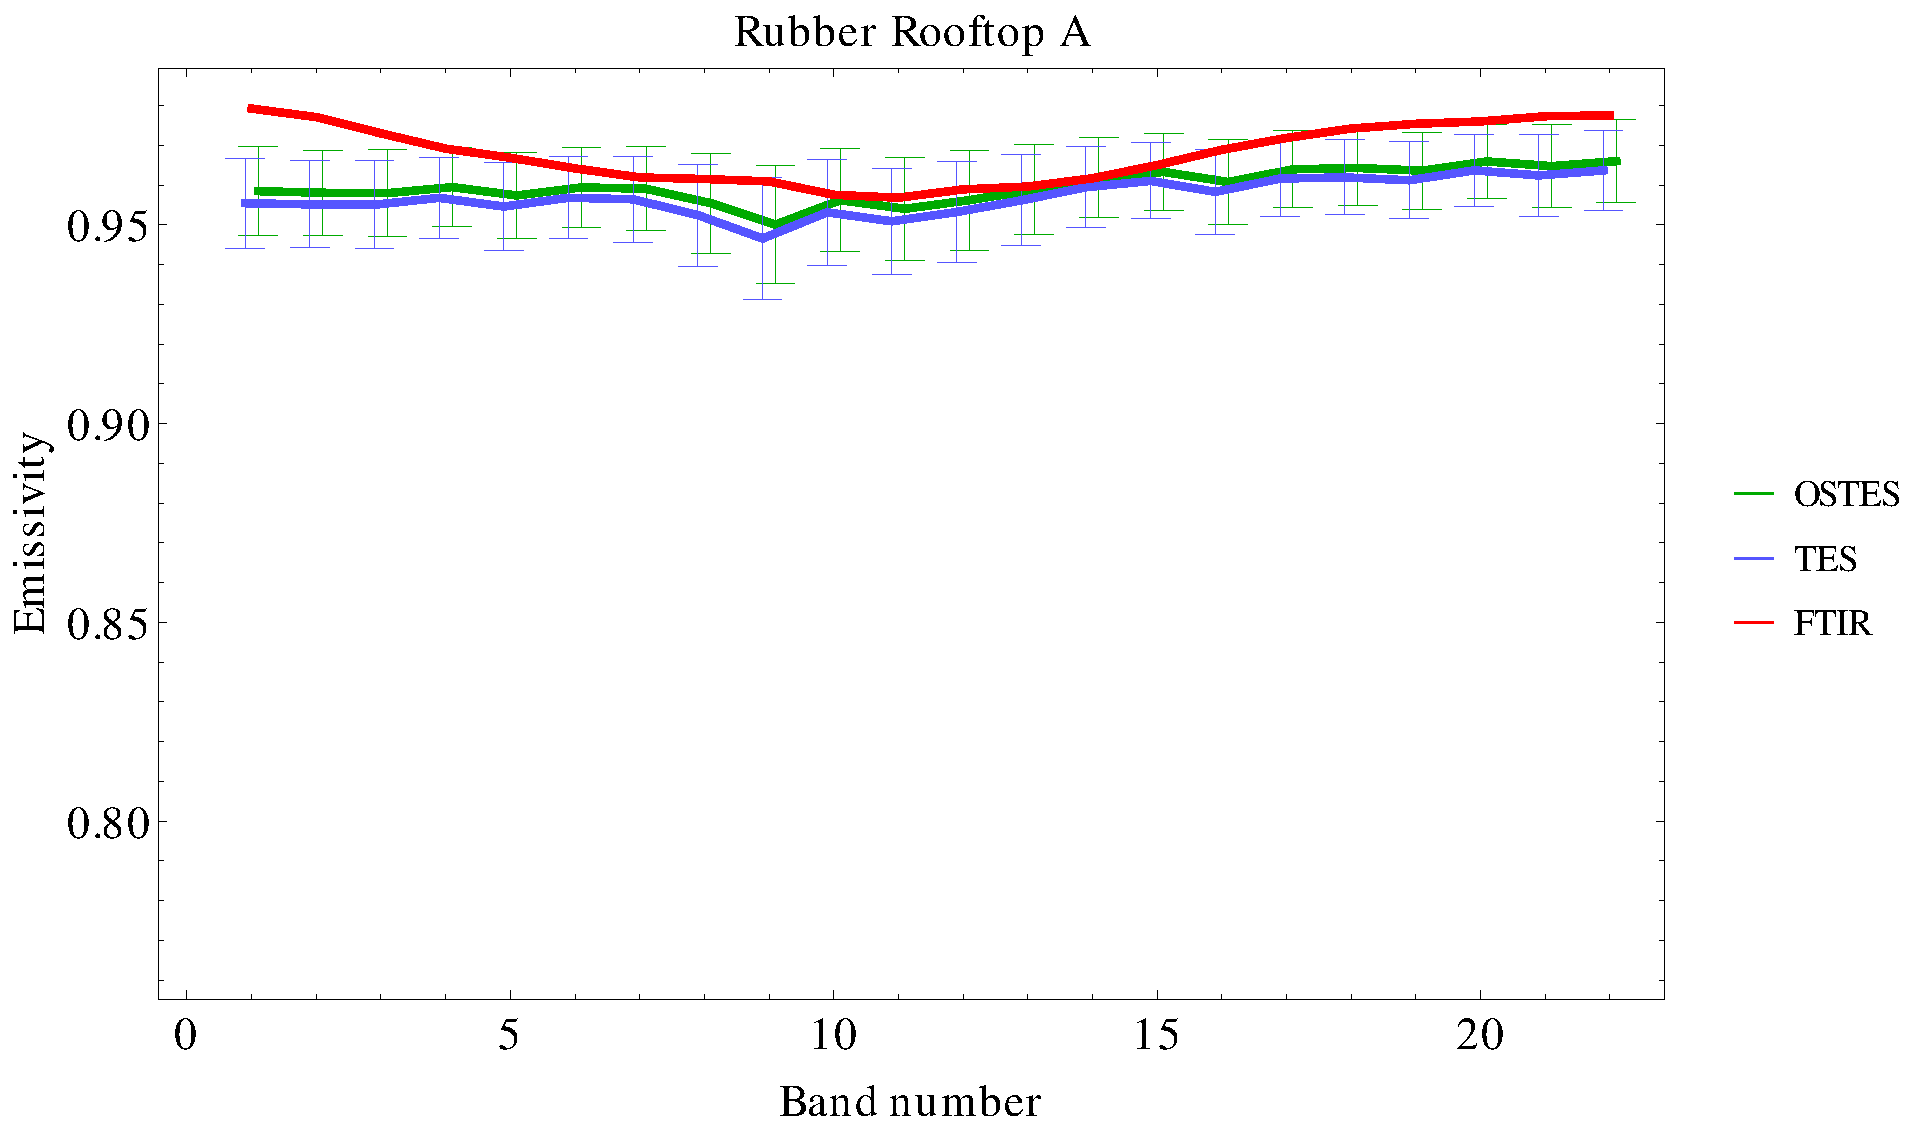
\includegraphics[scale=0.35]{RubberRooftopA.pdf}
\end{figure}
\end{frame}

\begin{frame}[plain]{}
\begin{figure}[htb]
	\centering
	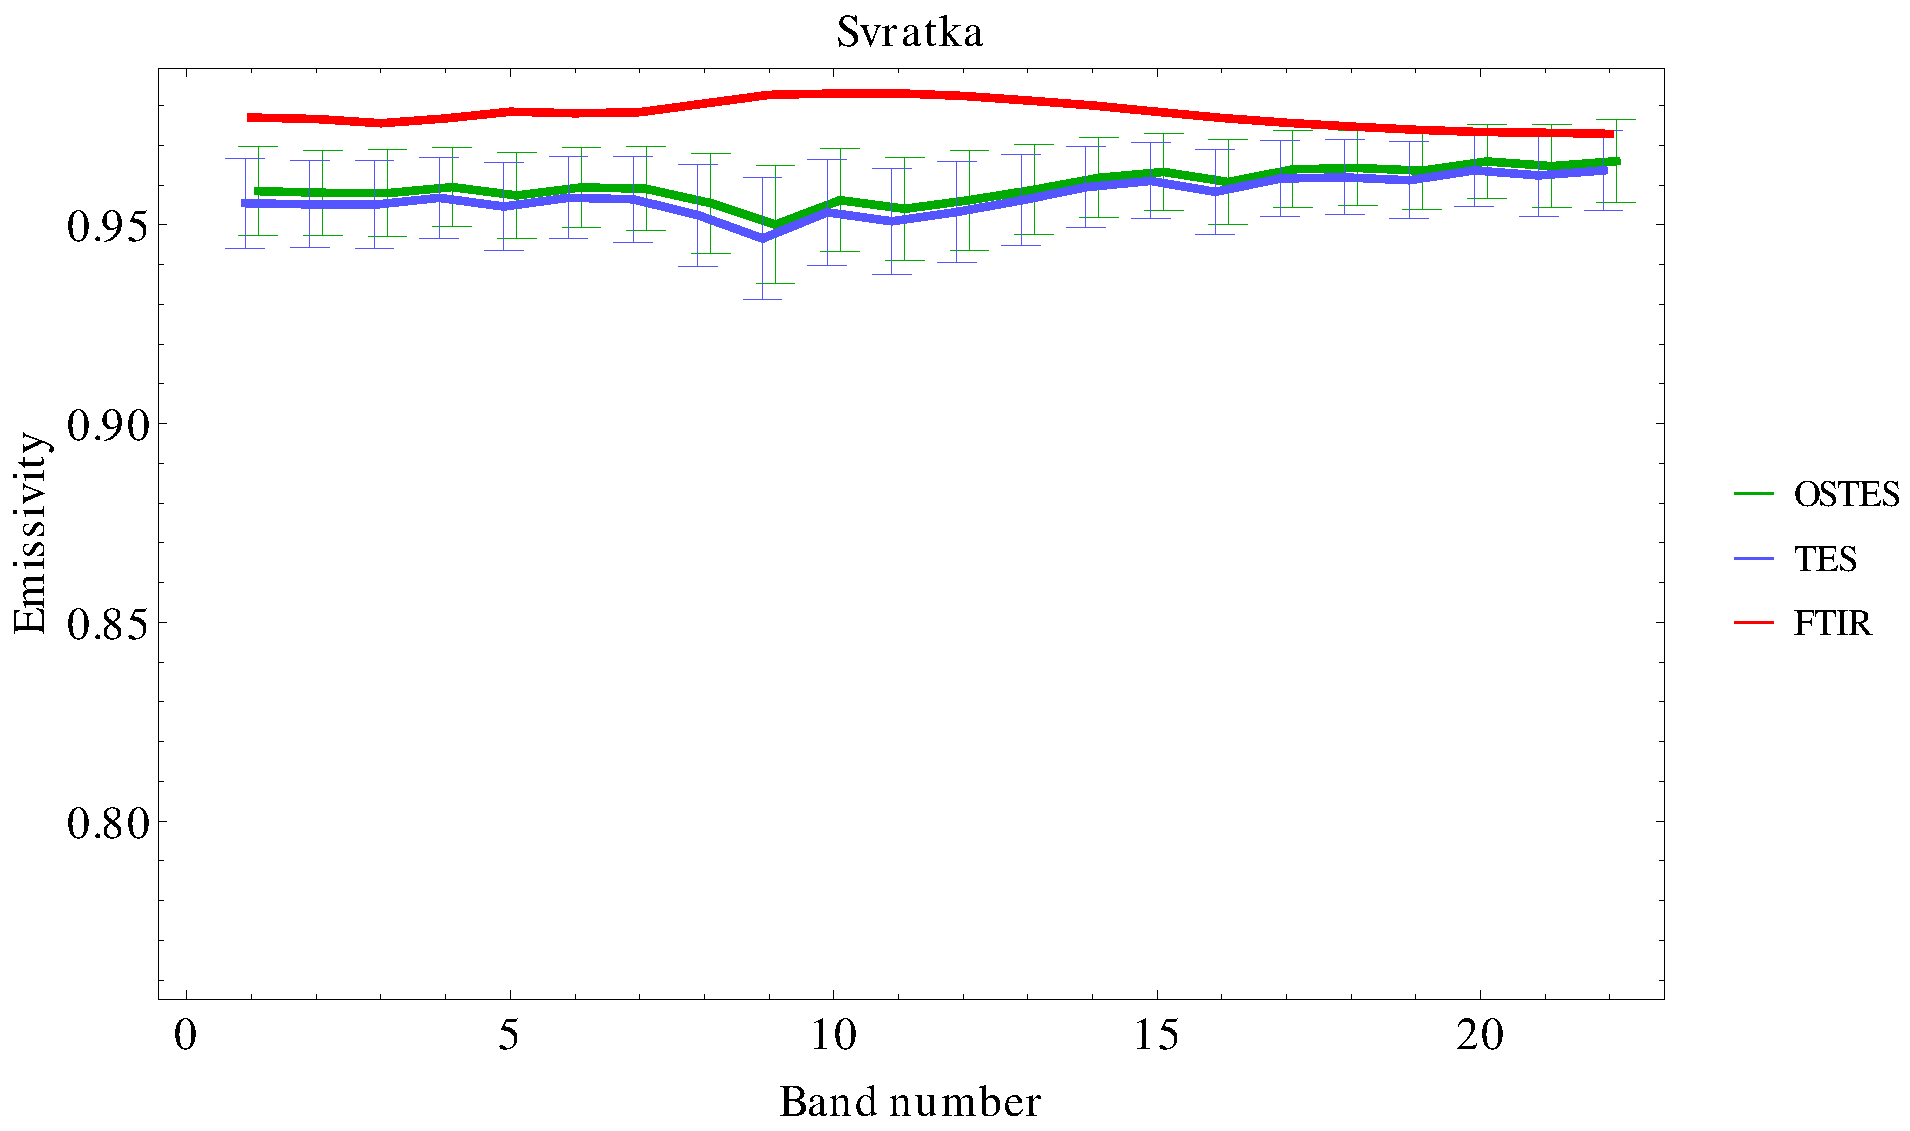
\includegraphics[scale=0.35]{Svratka.pdf}
\end{figure}
\end{frame}

\begin{frame}[plain]{}
\begin{figure}[htb]
	\centering
	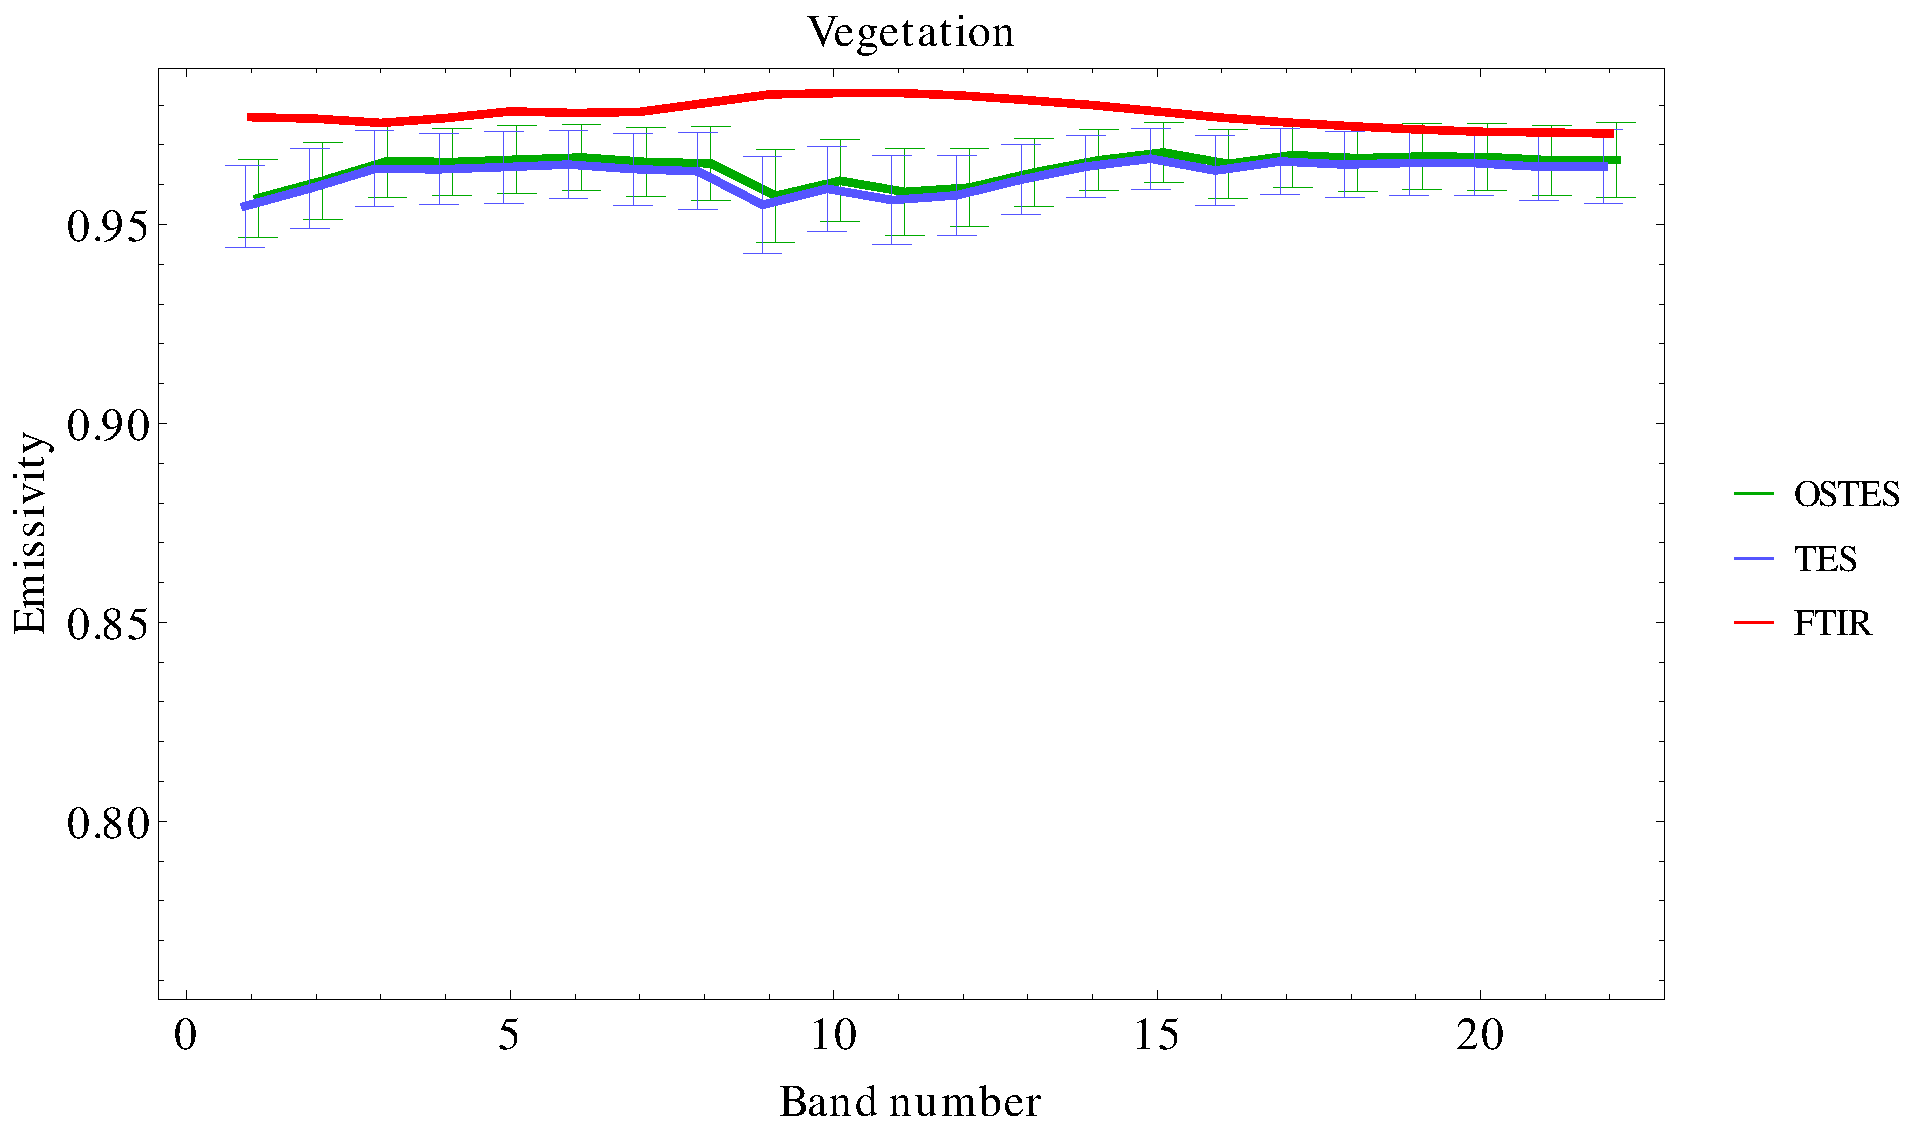
\includegraphics[scale=0.35]{Vegetation.pdf}
\end{figure}
\end{frame}

\begin{frame}[plain]{}
	\begin{center}
		\Huge\textsc{\Huge 2.}

		\textsc{\huge Scaled spectra}
	\end{center}
\end{frame}

\begin{frame}[plain]{}
\begin{figure}[htb]
	\centering
	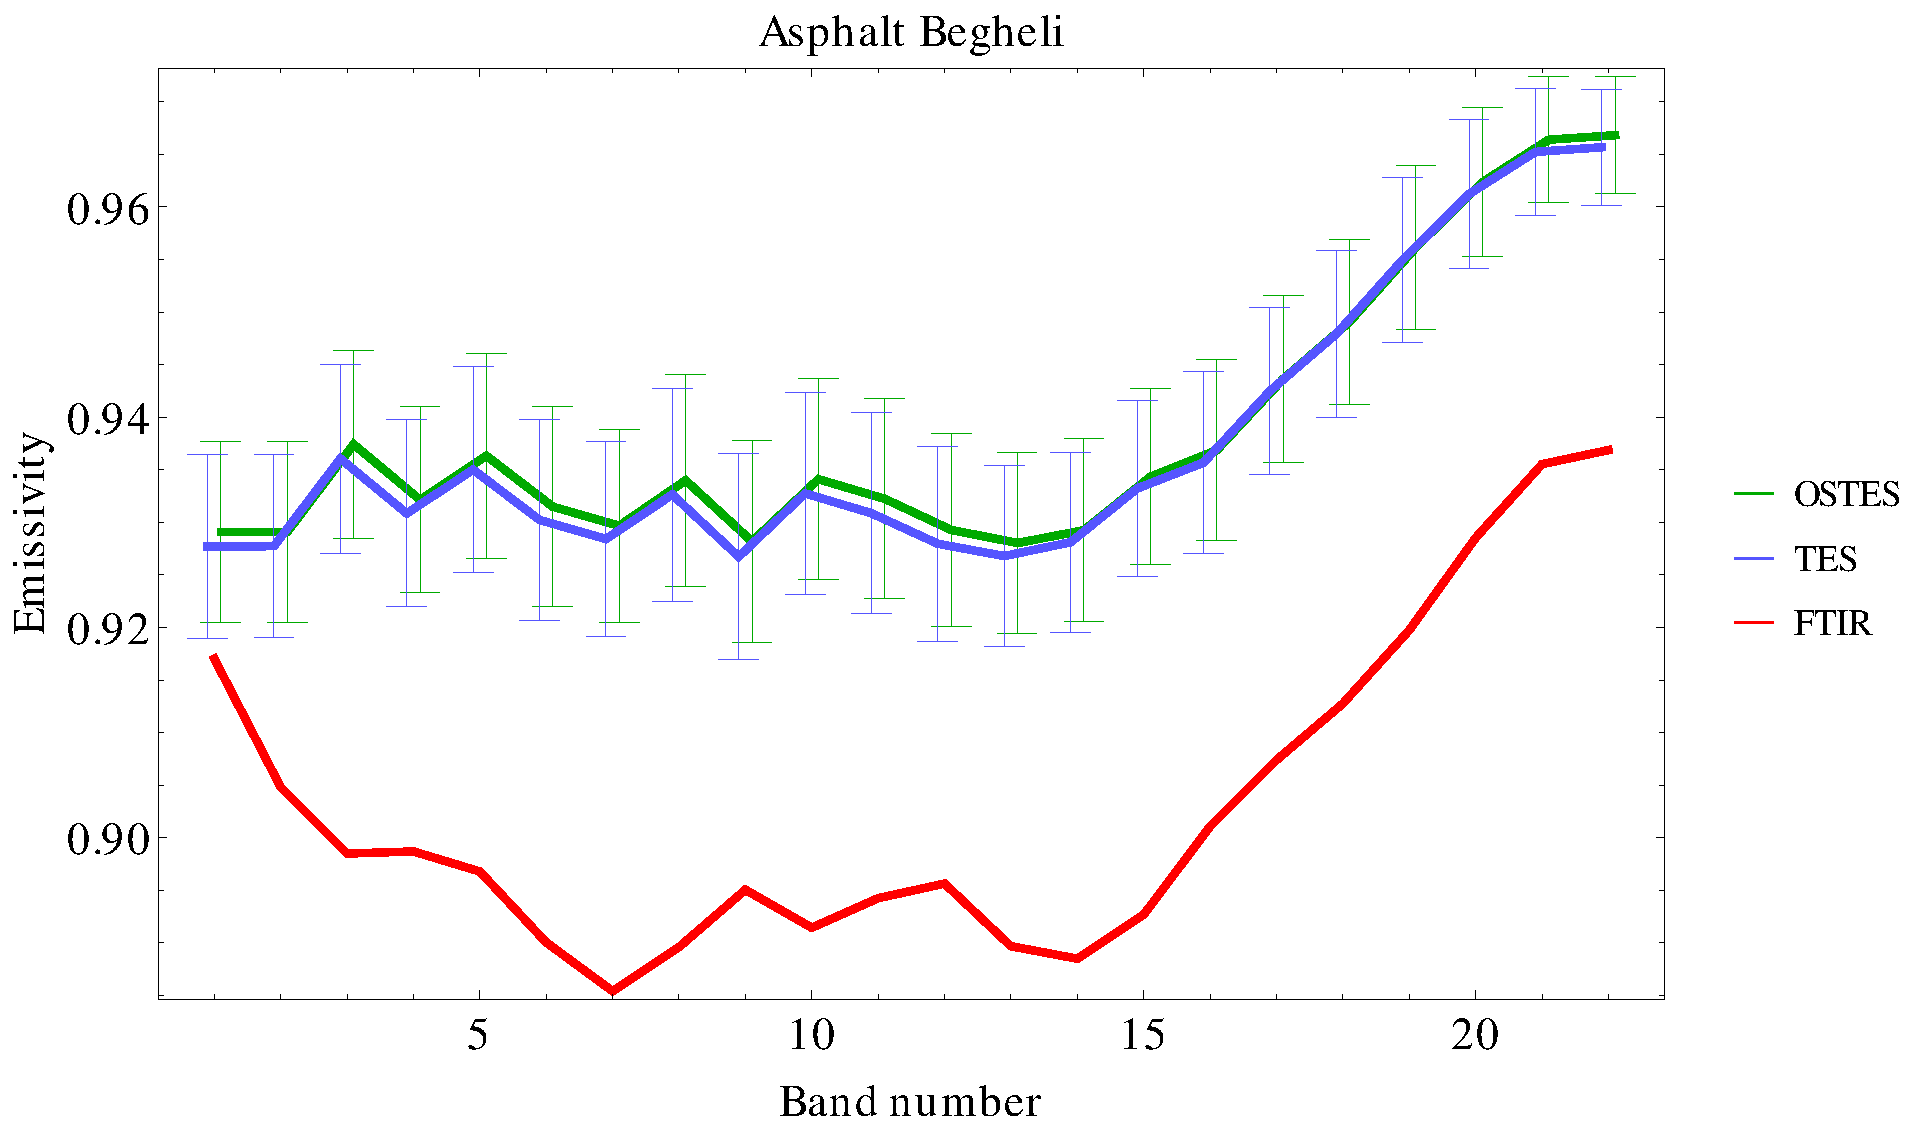
\includegraphics[scale=0.35]{AsphaltBegheli_scaled.pdf}
\end{figure}
\end{frame}

\begin{frame}[plain]{}
\begin{figure}[htb]
	\centering
	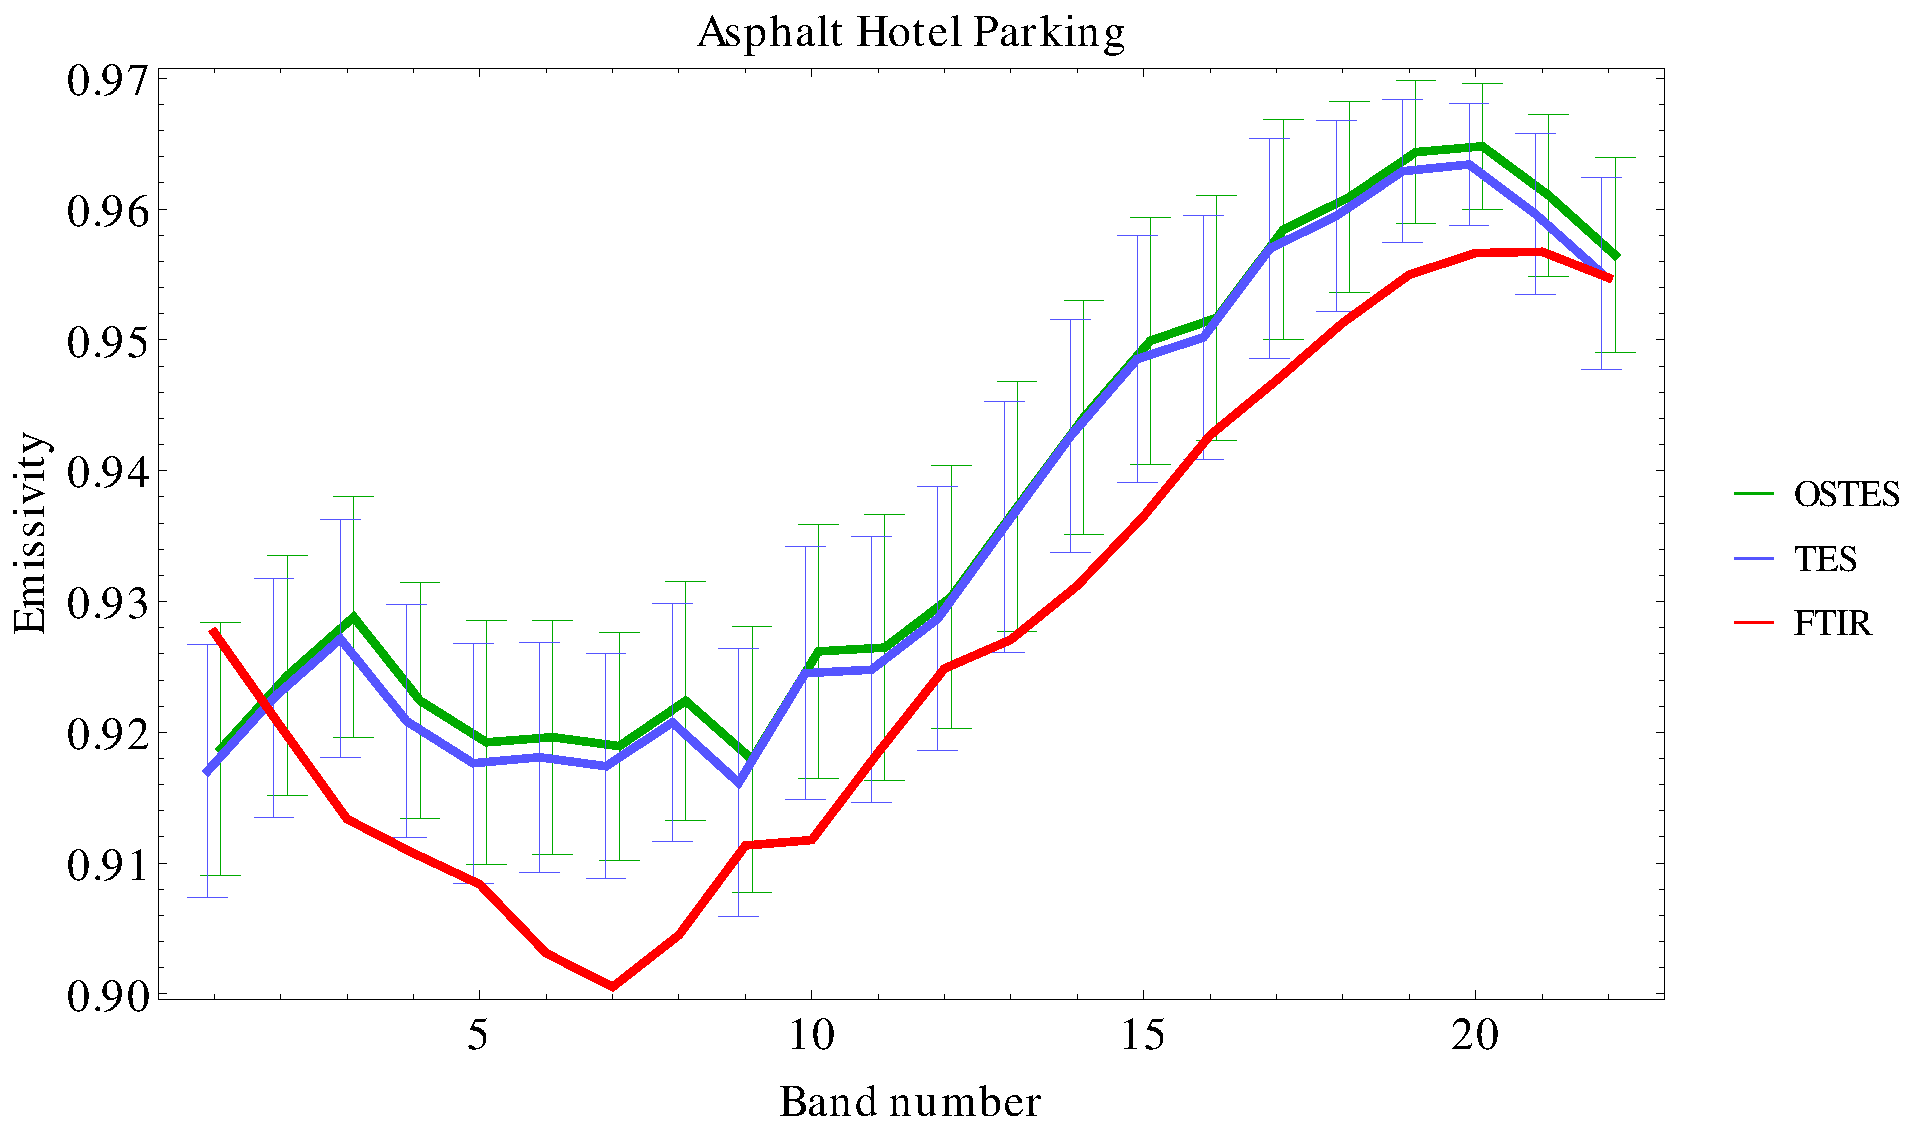
\includegraphics[scale=0.35]{AsphaltHotelParking_scaled.pdf}
\end{figure}
\end{frame}

\begin{frame}[plain]{}
\begin{figure}[htb]
	\centering
	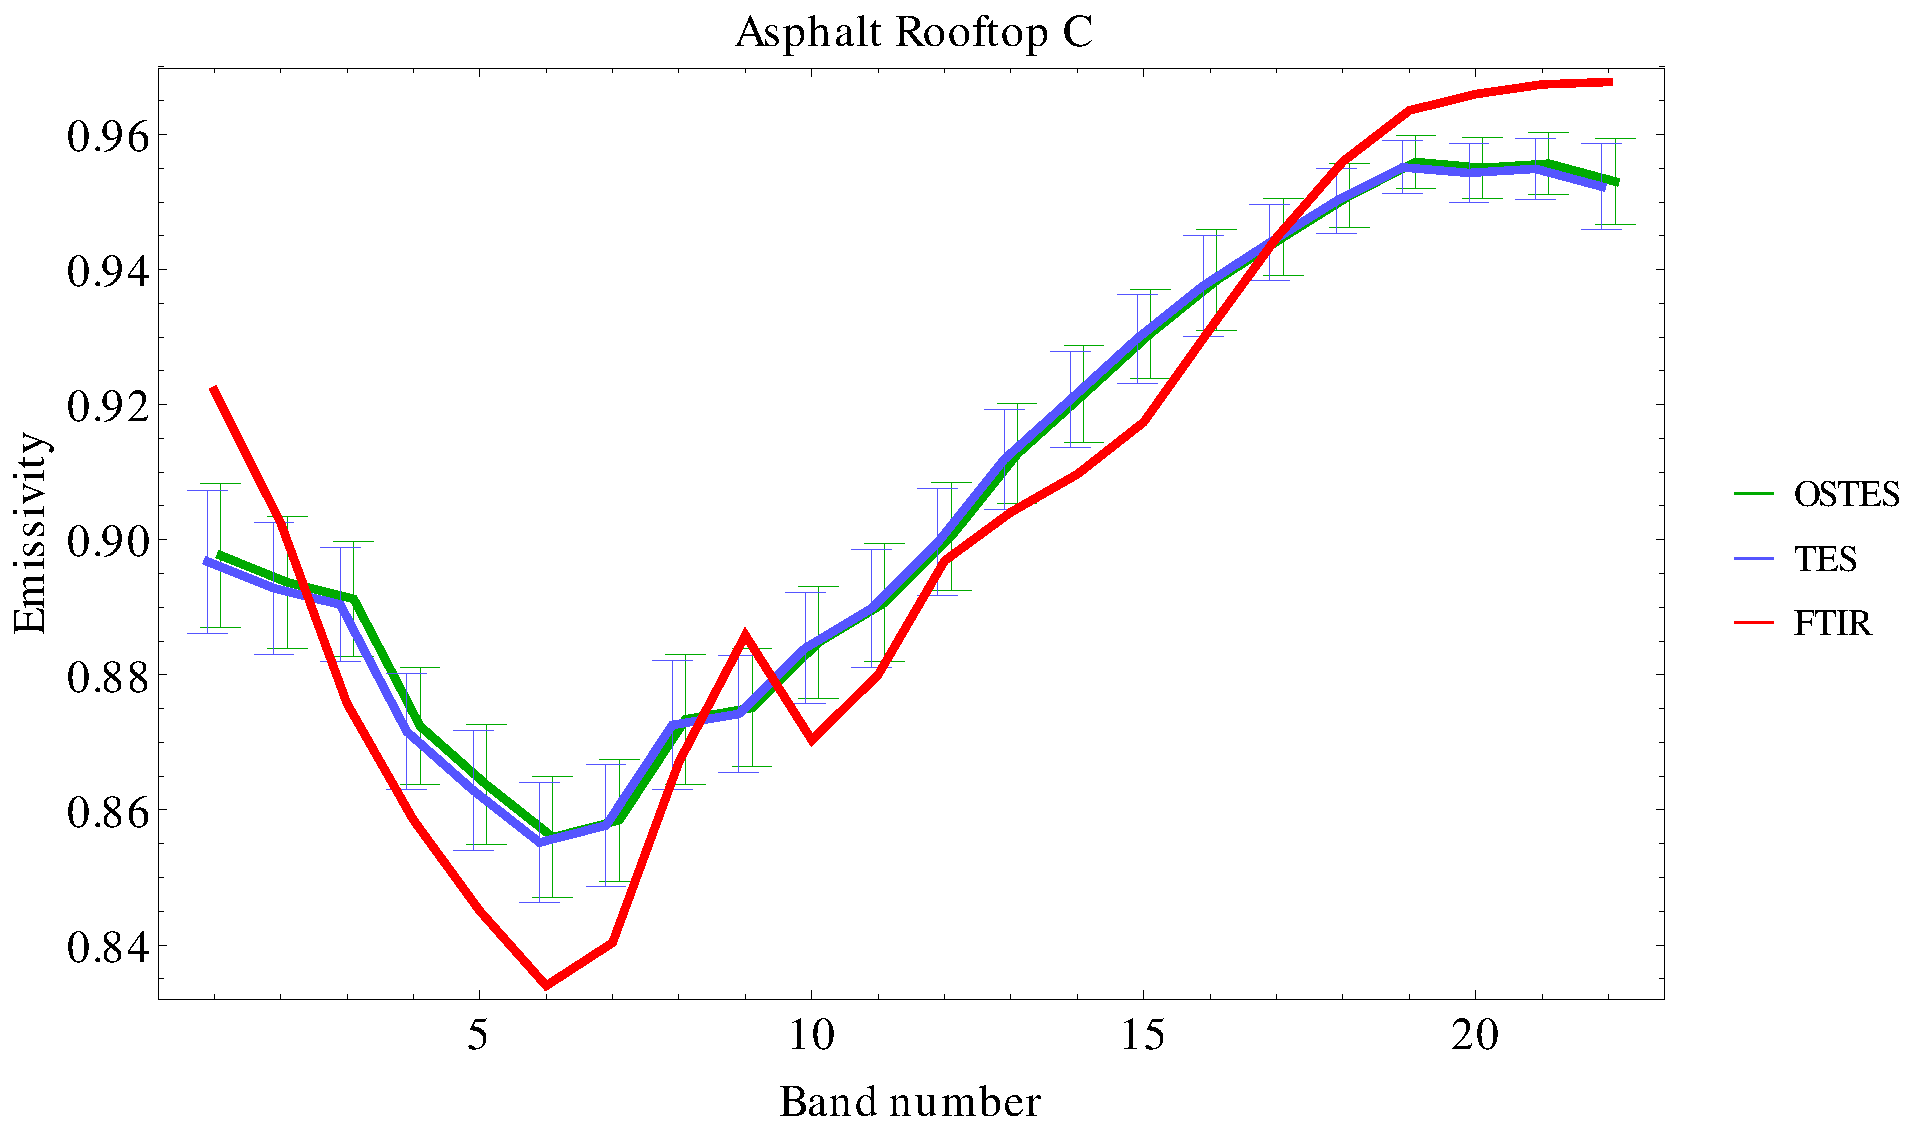
\includegraphics[scale=0.35]{AsphaltRooftopC_scaled.pdf}
\end{figure}
\end{frame}

\begin{frame}[plain]{}
\begin{figure}[htb]
	\centering
	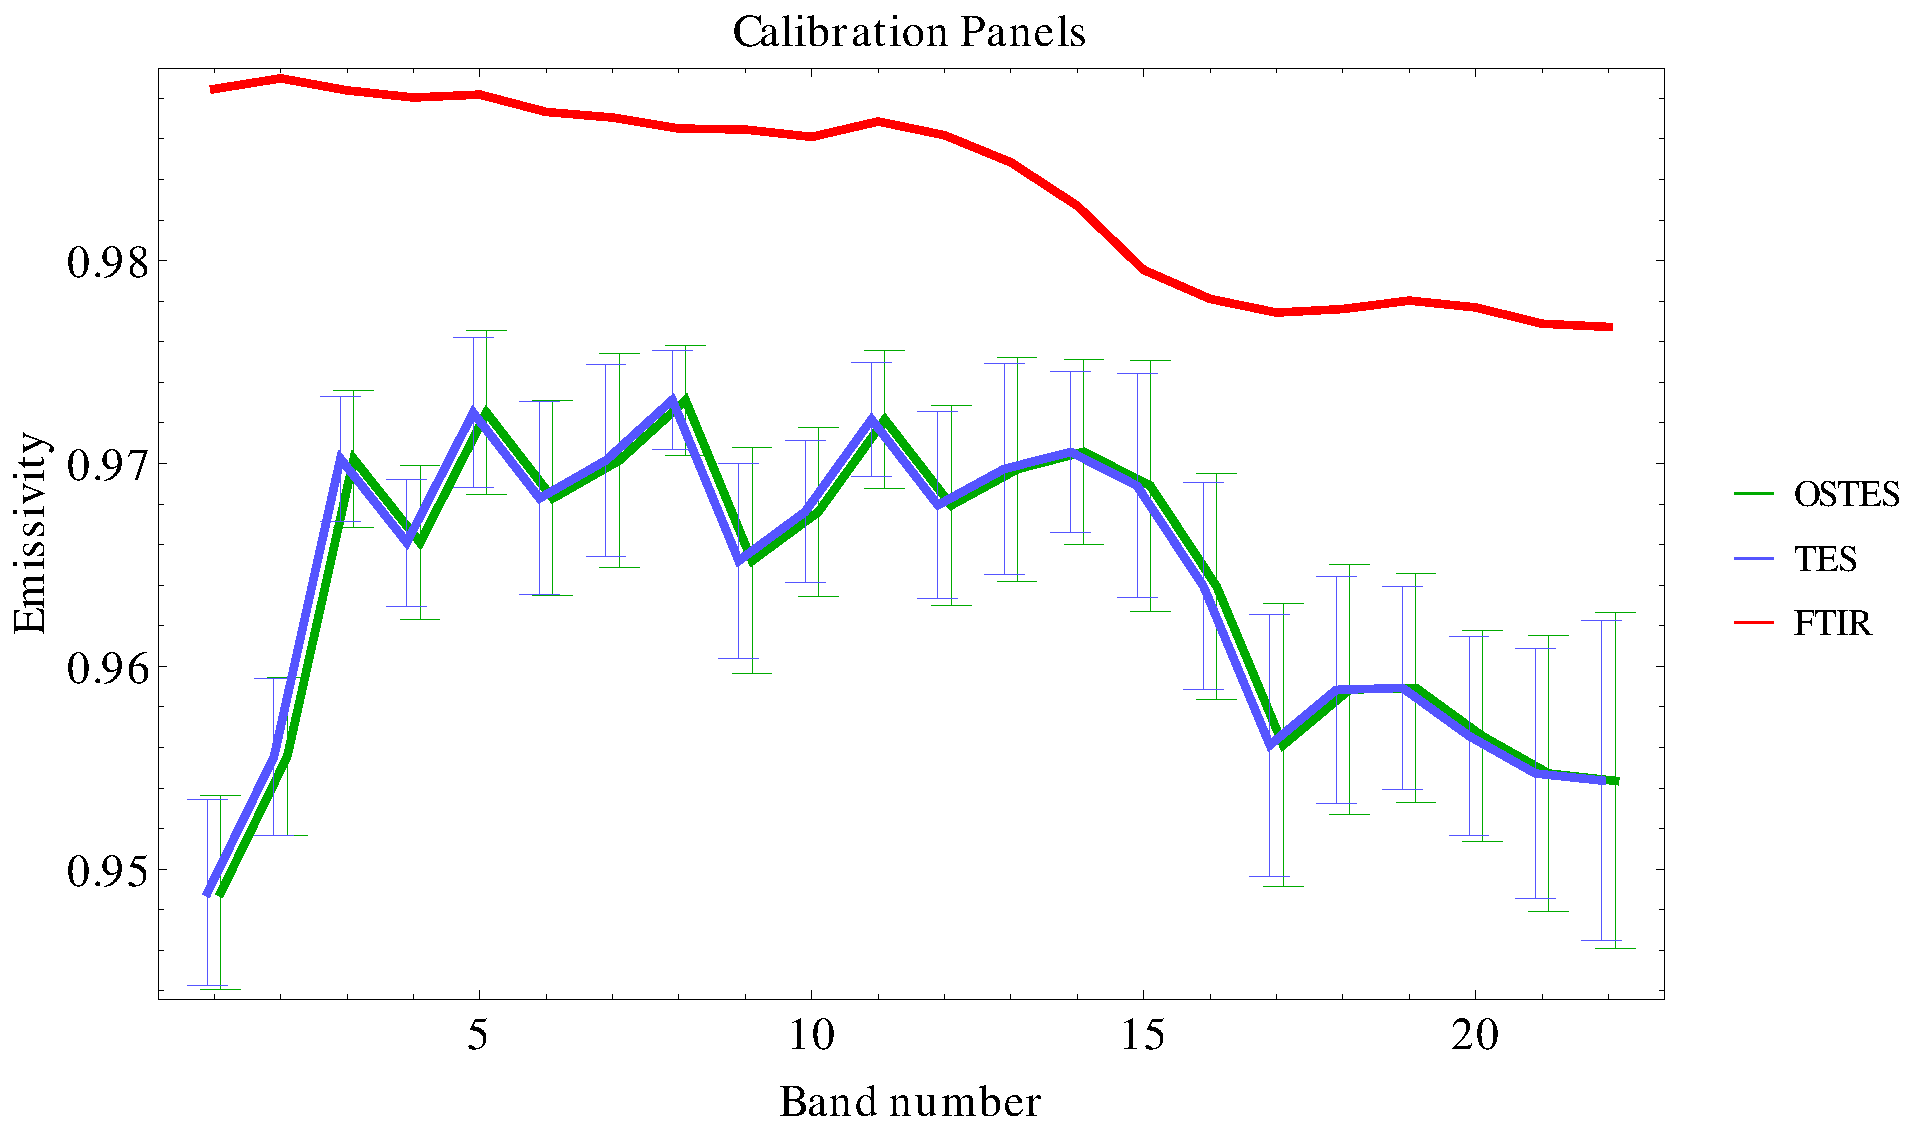
\includegraphics[scale=0.35]{CalibrationPanels_scaled.pdf}
\end{figure}
\end{frame}

\begin{frame}[plain]{}
\begin{figure}[htb]
	\centering
	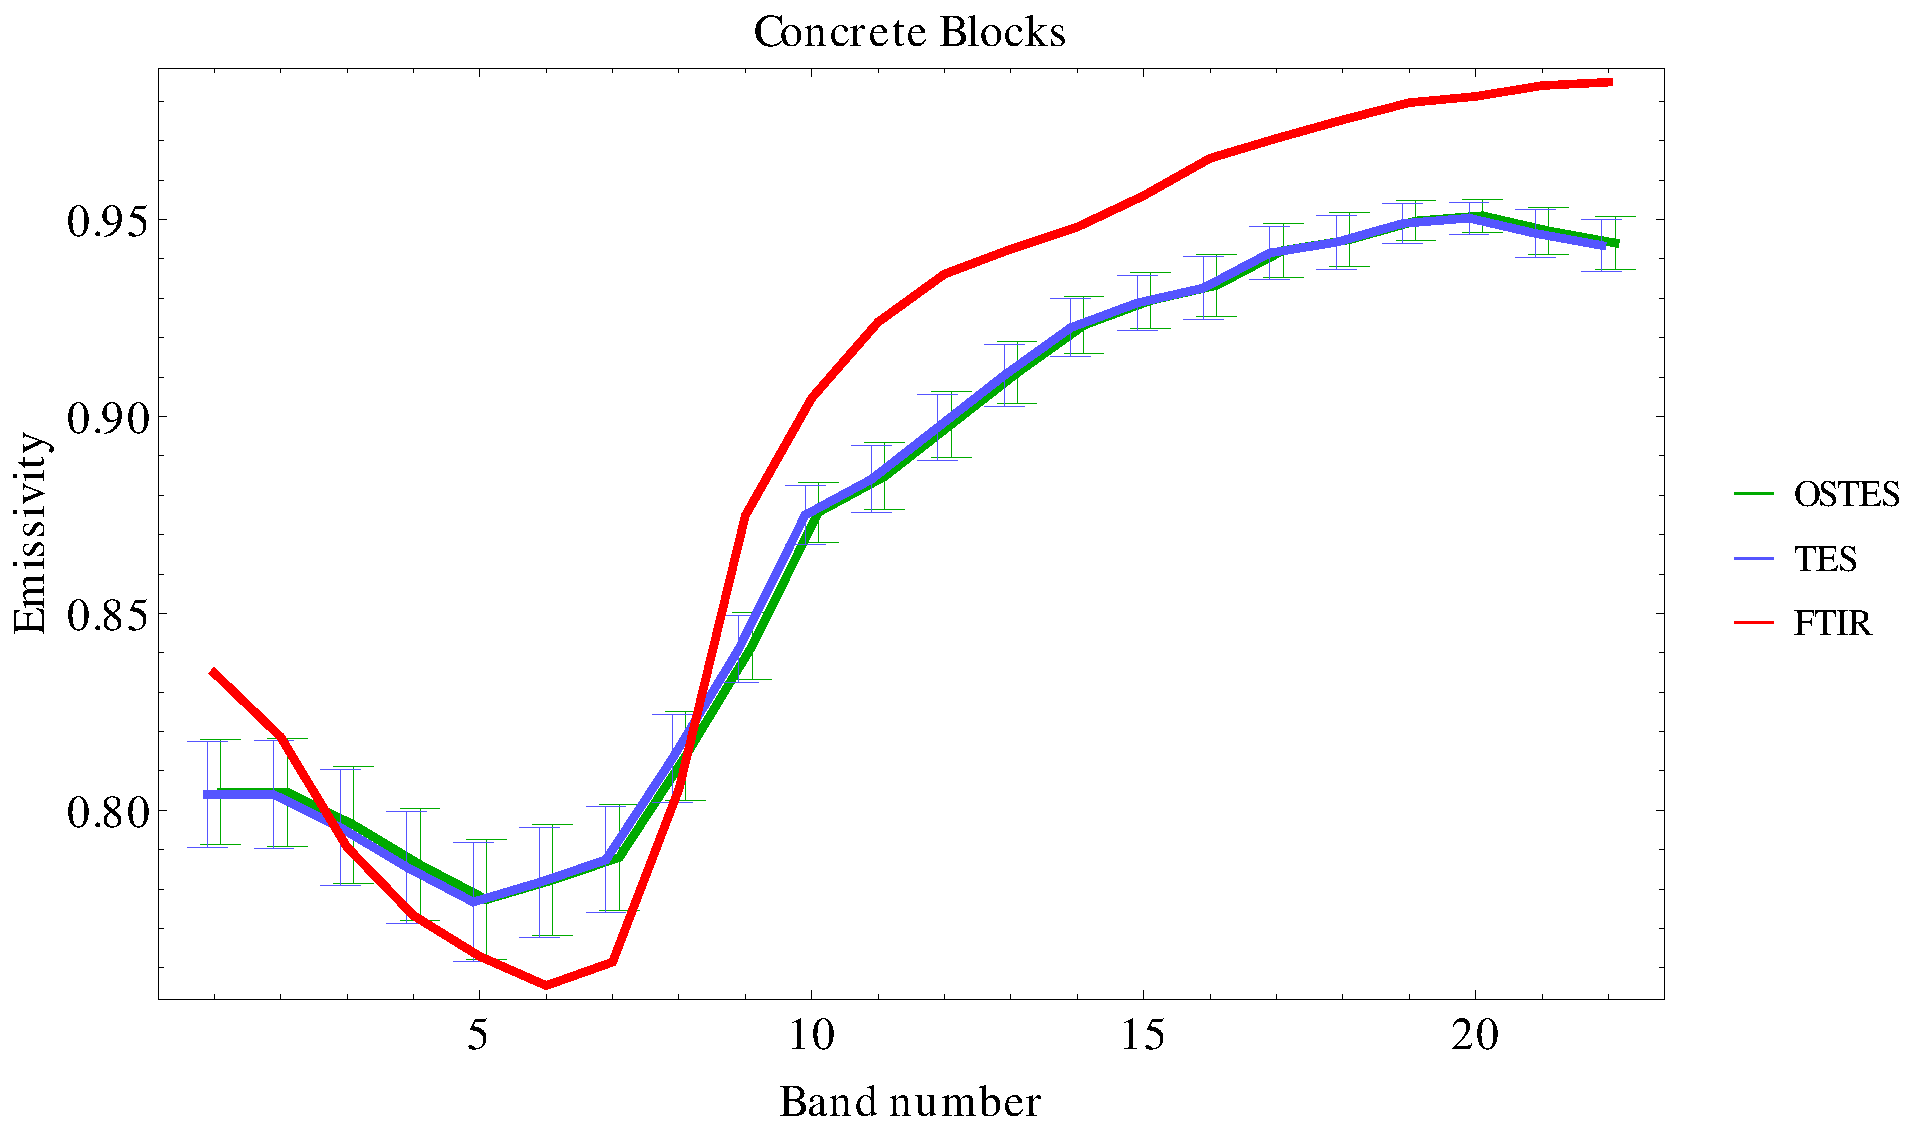
\includegraphics[scale=0.35]{ConcreteBlocks_scaled.pdf}
\end{figure}
\end{frame}

\begin{frame}[plain]{}
\begin{figure}[htb]
	\centering
	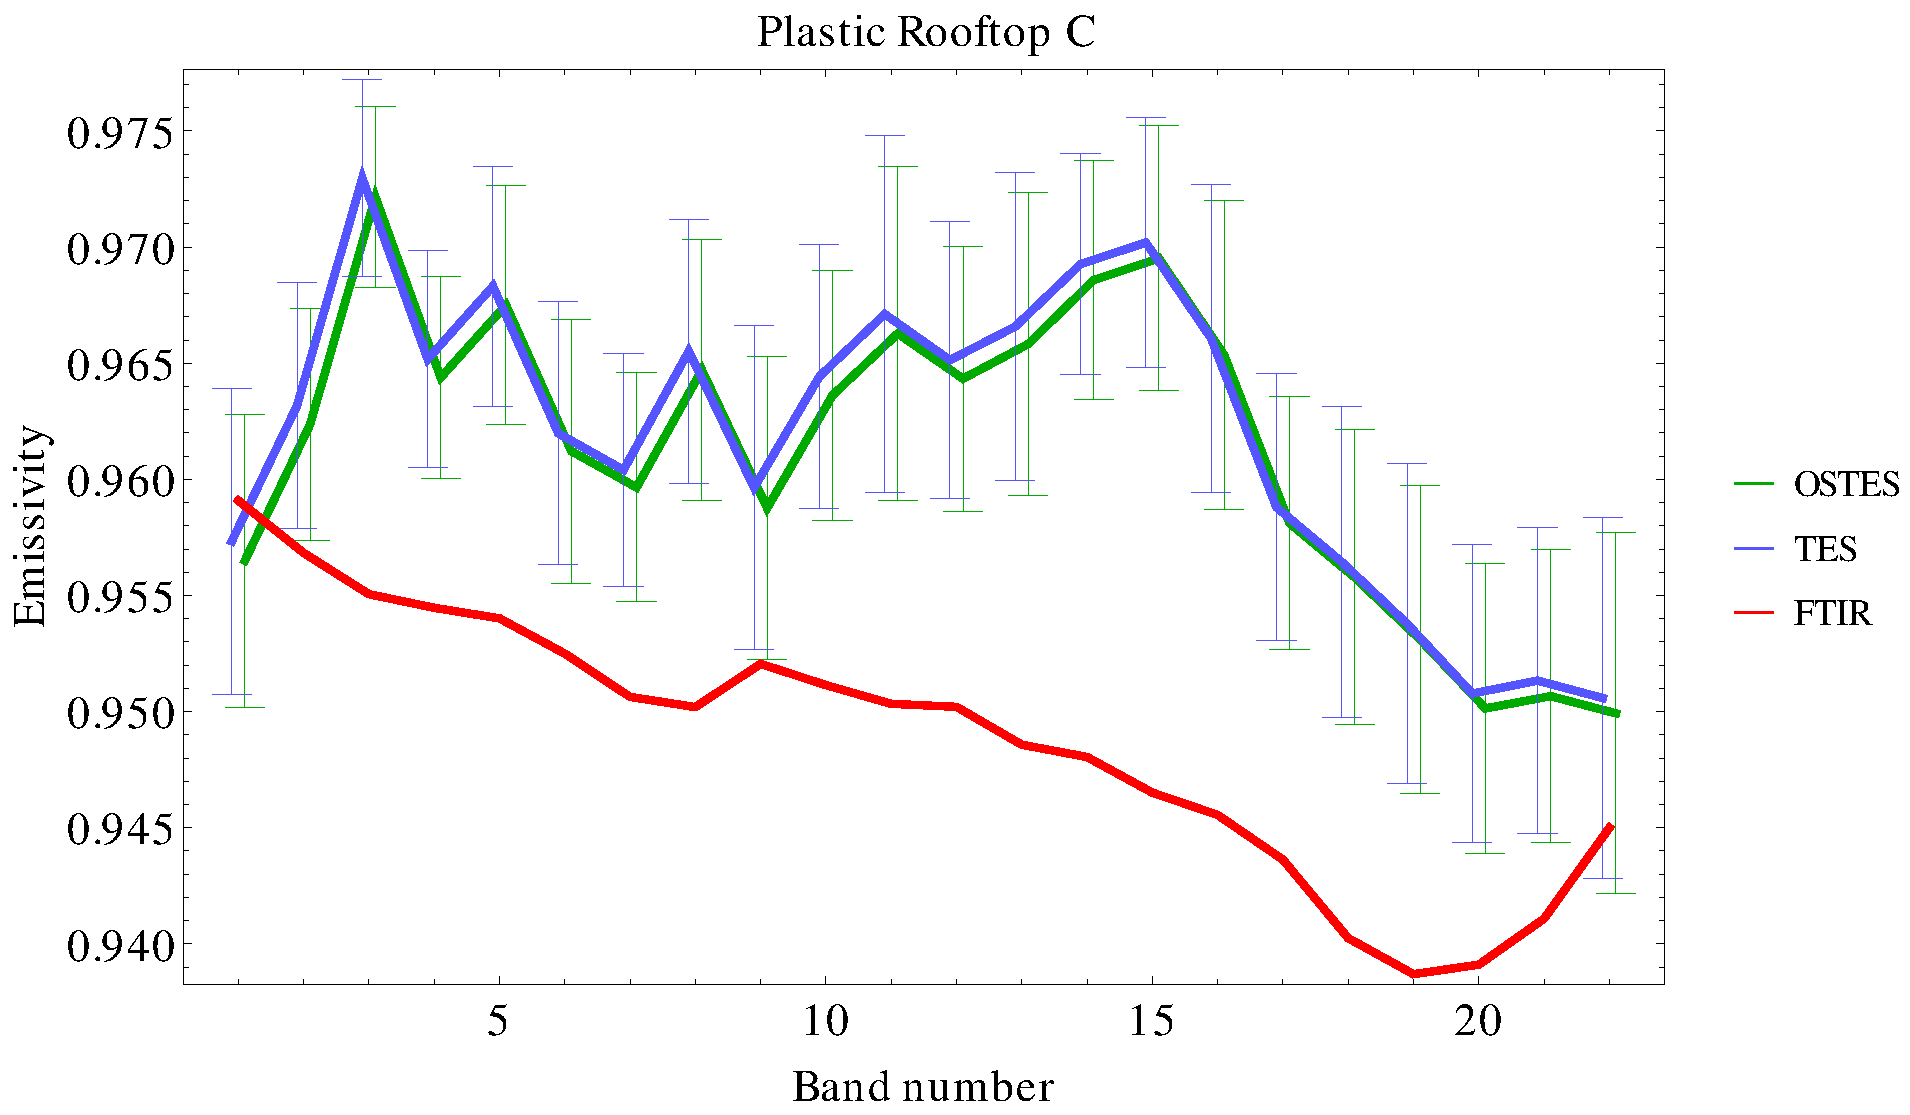
\includegraphics[scale=0.35]{PlasticRooftopC_scaled.pdf}
\end{figure}
\end{frame}

\begin{frame}[plain]{}
\begin{figure}[htb]
	\centering
	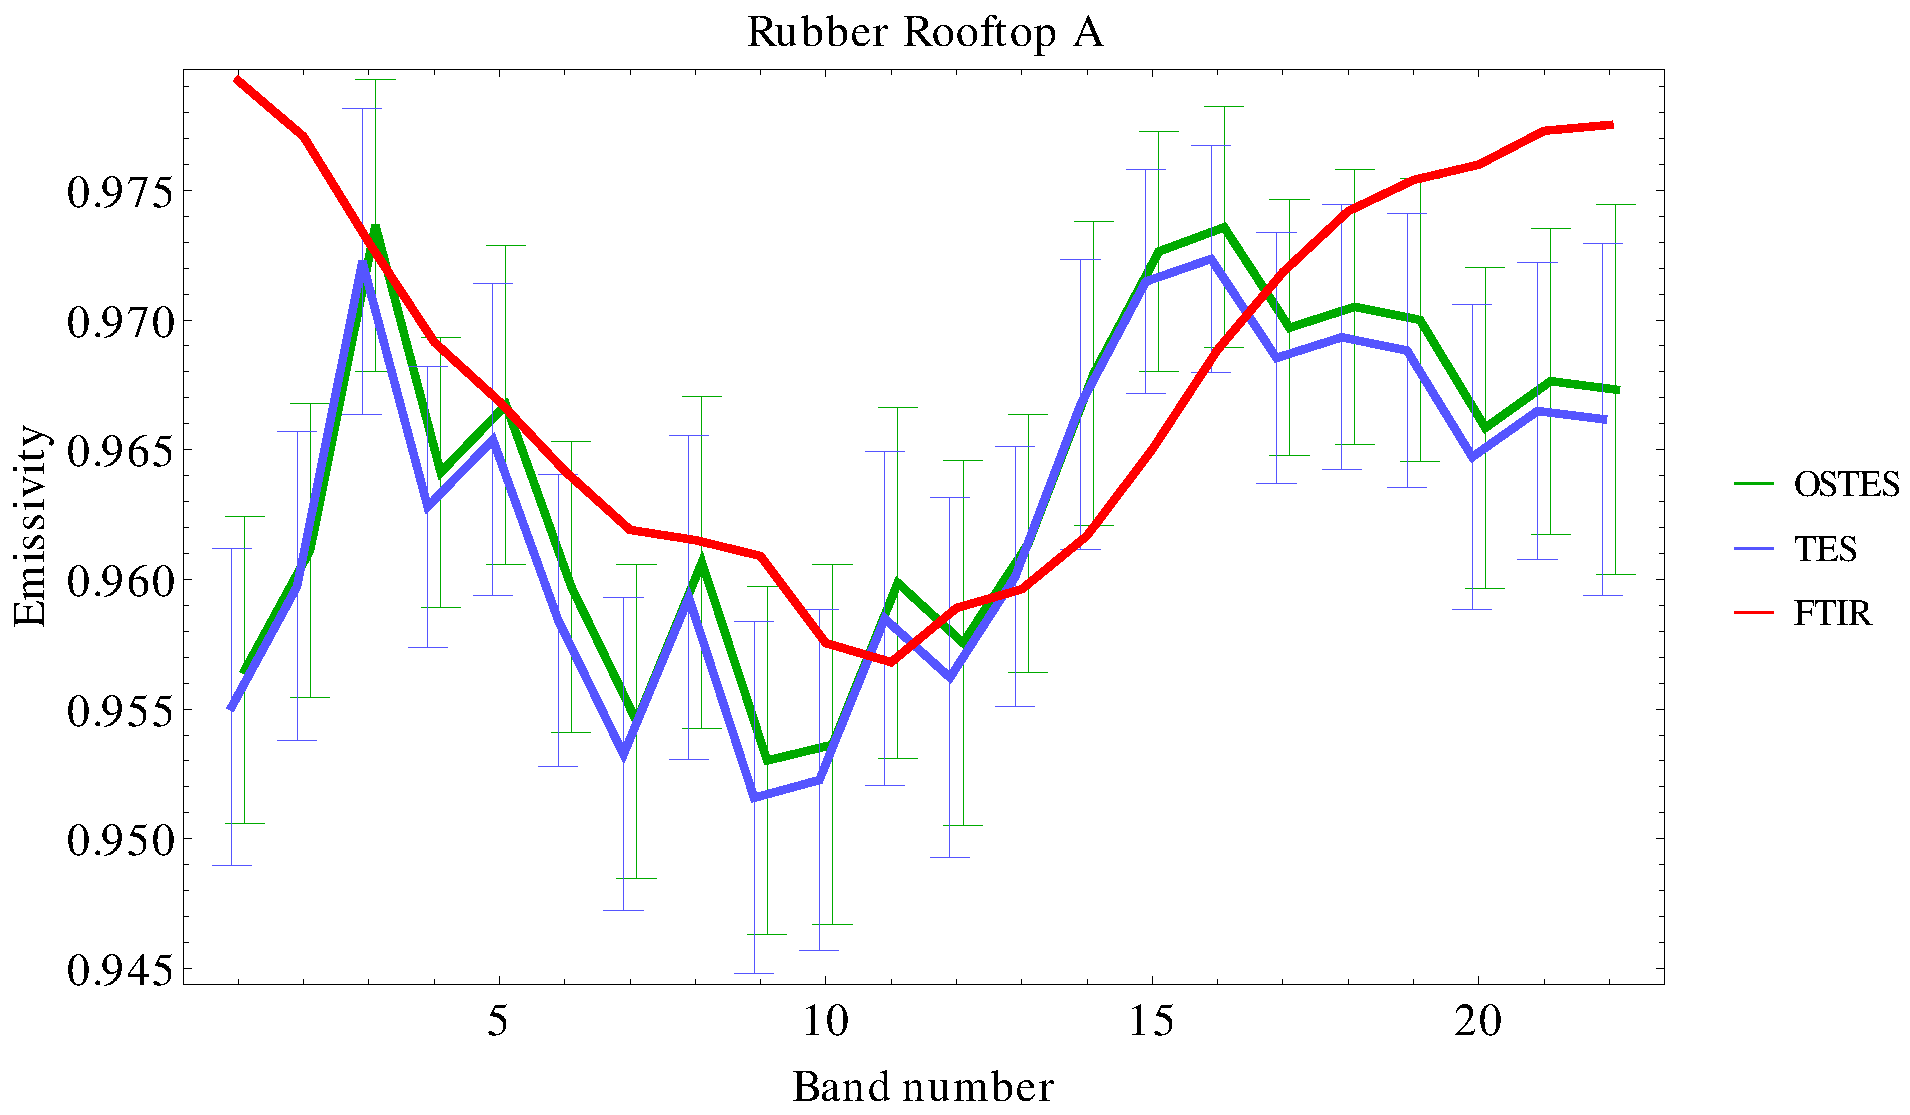
\includegraphics[scale=0.35]{RubberRooftopA_scaled.pdf}
\end{figure}
\end{frame}

\begin{frame}[plain]{}
\begin{figure}[htb]
	\centering
	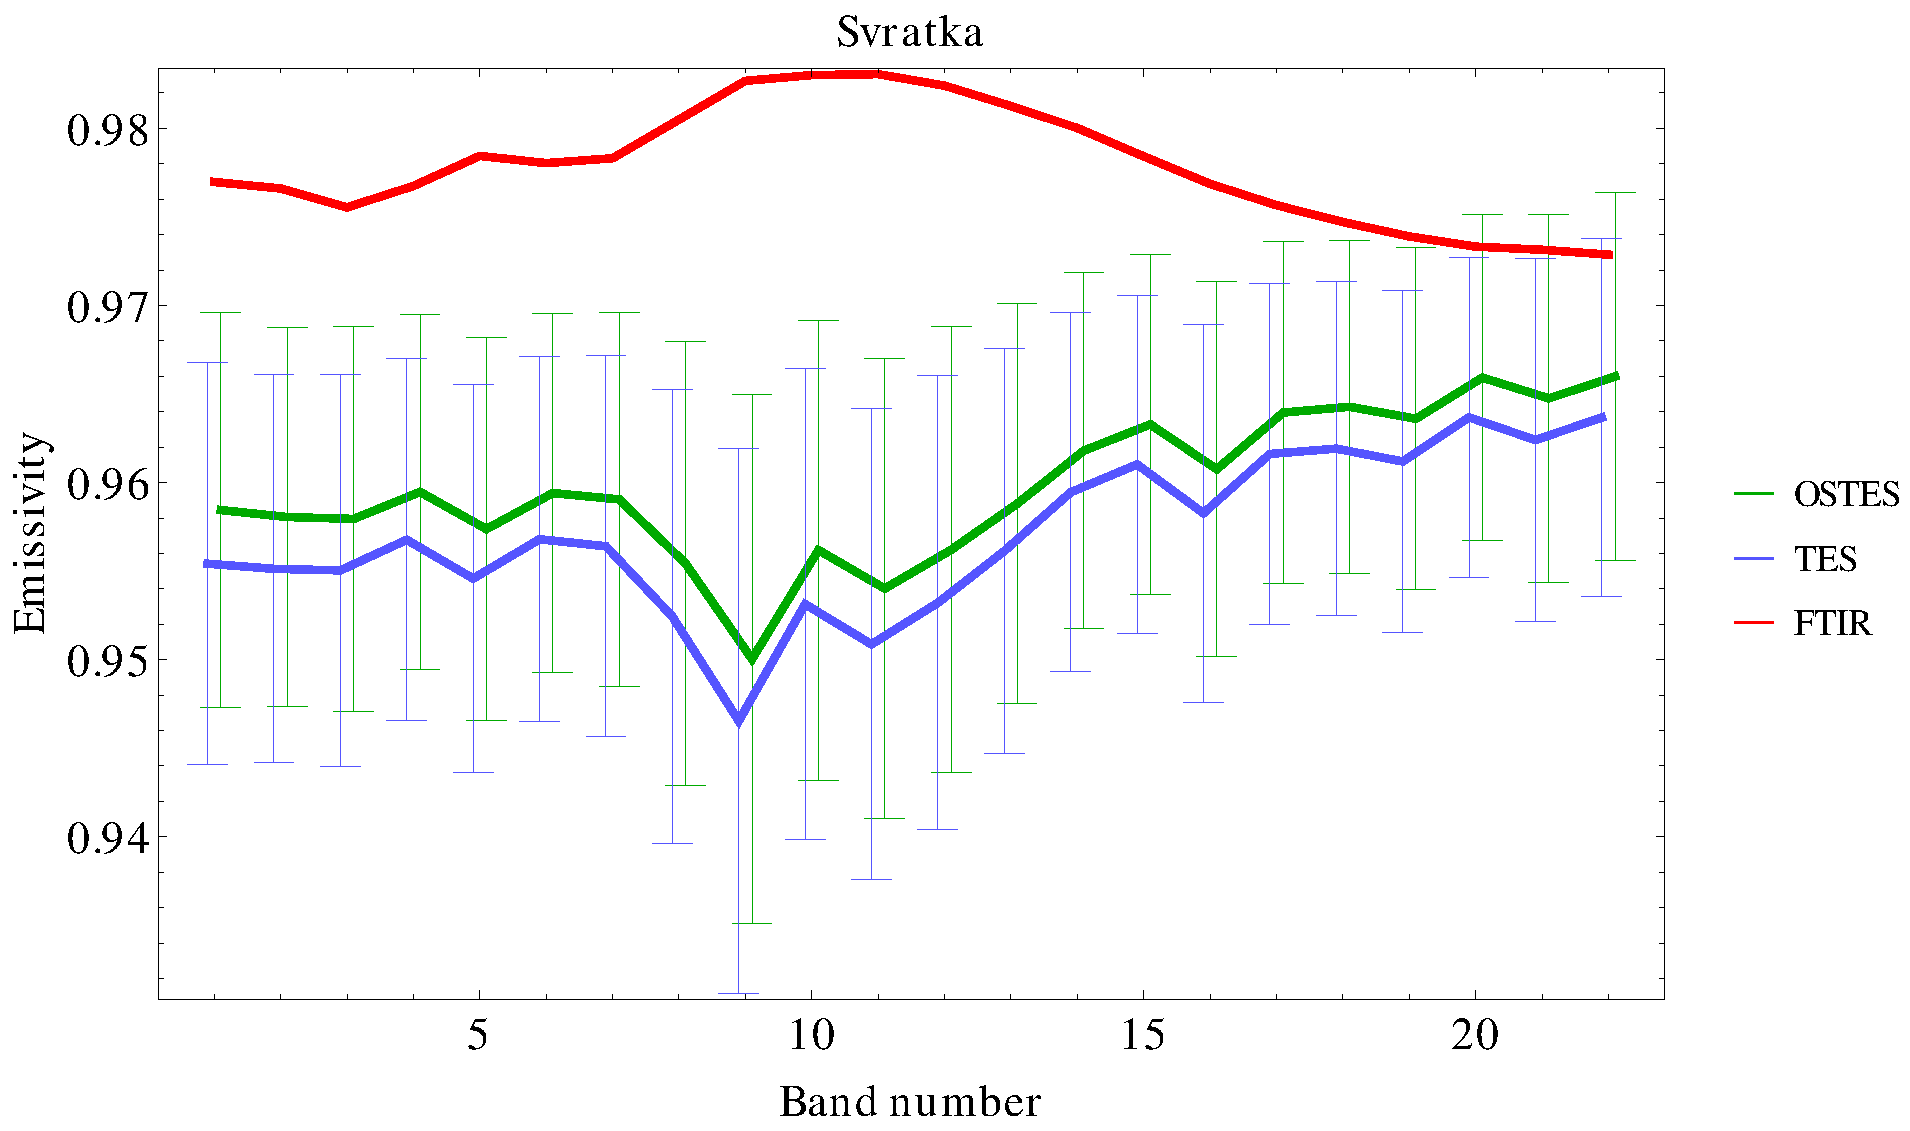
\includegraphics[scale=0.35]{Svratka_scaled.pdf}
\end{figure}
\end{frame}

\begin{frame}[plain]{}
\begin{figure}[htb]
	\centering
	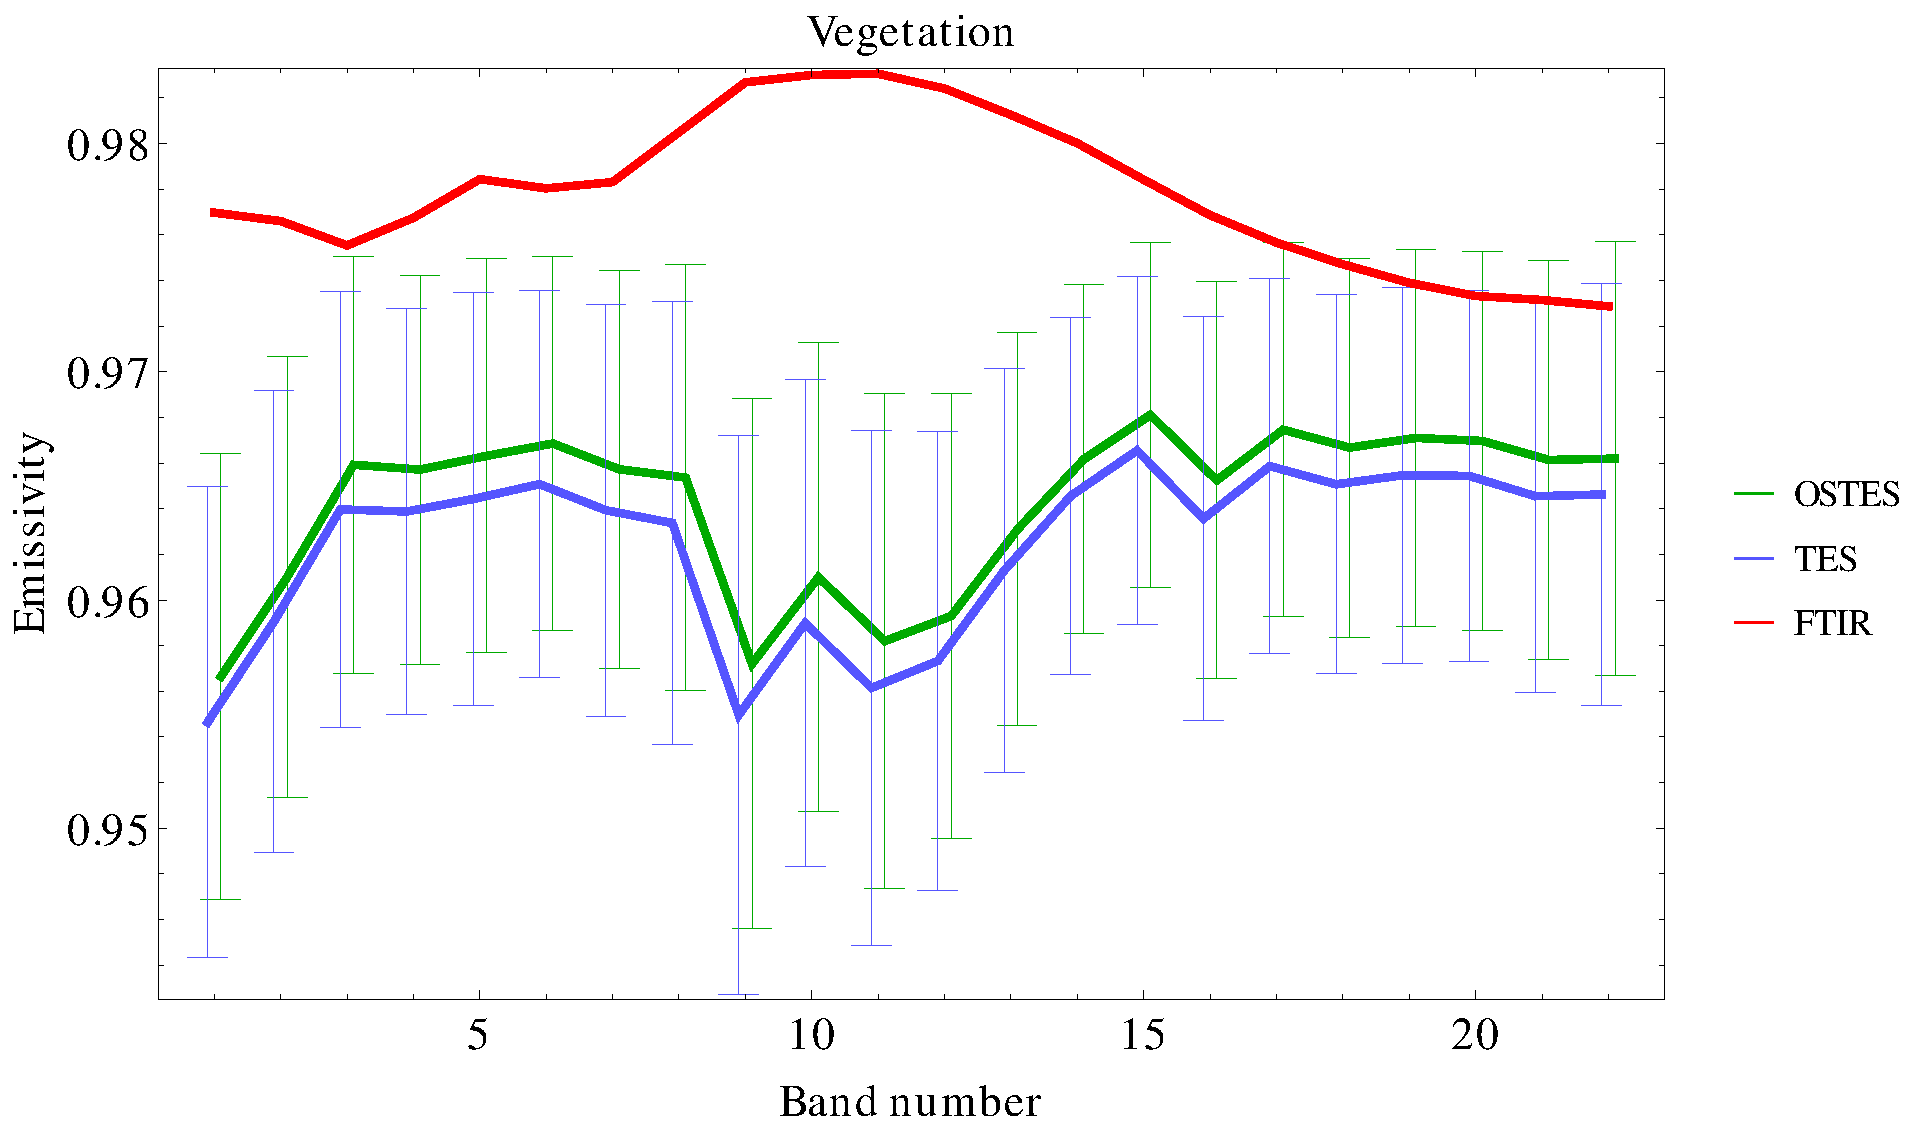
\includegraphics[scale=0.35]{Vegetation_scaled.pdf}
\end{figure}
\end{frame}

\end{document}